\chapter{Experiments and Results}

\section{Robot Planner 1: Simple MoveIt planning}
\label{section:robot-planner1}

In this first experiment we are testing some simple trajectories with the surgical tool already attached to the robot arm's end effector.
The path is designed using the appropriate coordinates and orientations so that the robot begins from the home position, then visits the table with the surgical 
tools and then visits the other table on top of which the mounting dock is placed. Upon arrival at the mounting dock, the robot inserts the tool inside a hole
(we consider these holes to be a simplistic alternative to the trocars used in real operations), then executes a simple pivot motion, while the tool is still 
inserted and then the tool gets ejected from the mounting dock's hole.\\

The aim of this experiment is to test the overall behaviour of the robot inside the work space, before implementing more complex path planning algorithms.

\begin{center}
\begin{figure}[!htb]
\centering
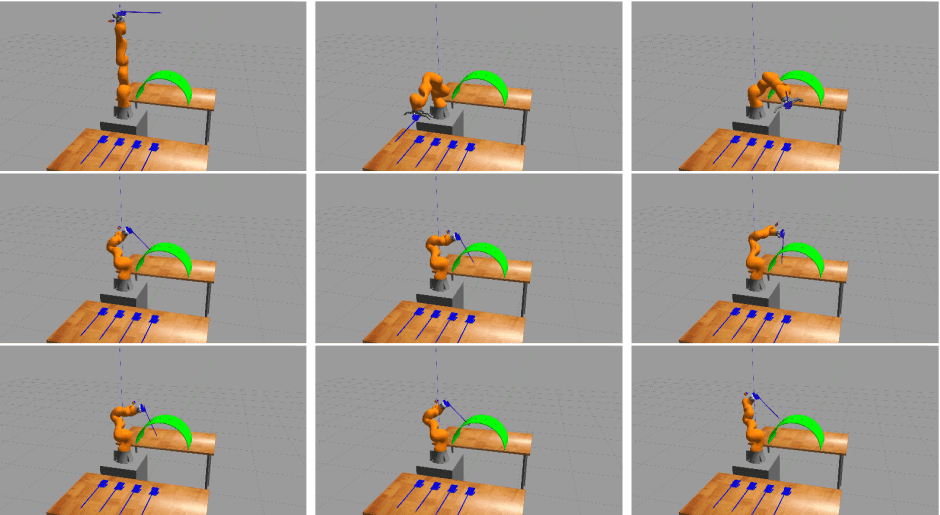
\includegraphics[width=\textwidth]{images/robot_planner1.png}
\caption{Experiment 1}
\end{figure}
\end{center}

% Robot Planner 1 with RRTConnect
\begin{table}[H]
\centering
\begin{tabular}{|p{2cm}|c|p{2cm}|p{2cm}|p{2cm}|}
\hline
Robot Planner 1           & \multicolumn{4}{c}{\textbf{RRTConnect}}                                                                                                 \vline \\
\hline
                          & \multicolumn{4}{c}{\textbf{Fake tool picking trajectory}}                     \vline \\
\hline
Experiment                & Approach planning time & Execution status & Move away planning time & Execution status  \\
\hline
1 &	0.060402 &	1 &	0.144881 &	1 \\
2 &	0.06053 &	1 &	0.058341 &	1 \\
3 &	0.064706 &	1 &	0.060981 &	1 \\
4 &	0.059789 &	1 &	0.119351 &	1 \\
5 &	0.164789 &	1 &	0.330373 &	1 \\
6 &	0.147037 &	1 &	0.289805 &	1 \\
7 &	0.18233 &	1 &	0.093362 &	1 \\
8 &	0.054469 &	1 &	0.062209 &	1 \\
9 &	0.05313 &	1 &	0.409191 &	1 \\
10 &	0.105909 &	1 &	0.307963 &	1 \\
\hline
\textbf{Average} & 	0.0953091 &	1	& 0.1876457	& 1 \\
\hline
\textbf{Standard deviation} & 	0.048230 &	- &	0.125796 & - \\
\hline
                          & \multicolumn{4}{c}{\textbf{Insertion \& Pivot trajectories}}                     \vline \\
\hline
Experiment                & Insertion planning time & Execution status & Pivot planning time & Execution status  \\
\hline
1	& 0.216565	& 1	& 3.639193	& 1 \\
2	& 0.057143	& 1	& 0.057187	& 1 \\
3	& 0.073242	& 1	& 0.072451	& 1 \\
4	& 0.056255	& 1	& 0.068156	& 1 \\
5	& 0.16178	& 1	& 0.150123	& 1 \\
6	& 0.071426	& 1	& 0.065059	& 1 \\
7	& 0.155125	& 1	& -	& 0 \\
8	& 0.315921	& 1	& 0.194663	& 1 \\
9	& 0.127381	& 1	& 0.19026	& 1 \\
10	& 0.396182	& 1	& 0.075866	& 1 \\
\hline
\textbf{Average} & 	0.163102 & 1	& 0.5014398 &	0.9 \\
\hline
\textbf{Standard deviation} & 	0.110001 &	- &	1.110582 & - \\
\hline
                          & \multicolumn{4}{c}{\textbf{Reverse pivot \& retraction trajectories}}                     \vline \\
\hline
Experiment                & Reverse pivot planning time & Execution status & retraction planning time & Execution status  \\
\hline
1 & 2.419514	& 1	& 2.388166	& 1 \\
2 & 1.386188	& 1	& 2.874223	& 0 \\
3 & -	& 0	& 5.106926	& 1 \\
4 & 5.466561	& 1	& 4.562506	& 1 \\
5 & 5.62329	& 1	& 5.587679	& 1 \\
6 & 5.488728	& 0	& -	& 0 \\
7 & -	& 0	& -	& 0 \\
8 & -	& 0	& -	& 0 \\
9 & 5.291442	& 1	& 5.096234	& 1 \\
10 & 5.381595	& 1	& 5.576362	& 1 \\
\hline
\textbf{Average} & 	4.436760	& 0.6	& 4.456014	& 0.6 \\
\hline
\textbf{Standard deviation} & 	1.628910 &	- &	1.204682 & - \\
\hline
\end{tabular}
\caption{Time results for robot planner 1 using the RRTConnect path planner algorithm. Planning time is the sum of solution time and path simplification time. Execution status is 
1 for success and 0 for failure. Parameters: tolerances: 0.000005, max planning time: 5 seconds, replanning: true, max planning attempts: 6. Experiments start from home position.}
\label{robot-planner1-rrtconnect-data}
\end{table}


% Robot Planner 1 with RRT*
\begin{table}[H]
\centering
\begin{tabular}{|p{2cm}|c|p{2cm}|p{2cm}|p{2cm}|}
\hline
Robot Planner 1           & \multicolumn{4}{c}{\textbf{RRT*}}                                                                                                 \vline \\
\hline
                          & \multicolumn{4}{c}{\textbf{Fake tool picking trajectory}}                     \vline \\
\hline
Experiment                & Approach planning time & Execution status & Move away planning time & Execution status  \\
\hline
1	& 5.096772	& 1	& 5.023175	& 1 \\
2	& 5.015857	& 1	& 5.034447	& 1 \\
3	& 5.01843	& 1	& 5.101766	& 1 \\
4	& 5.074703	& 1	& 5.089464	& 1 \\
5	& 5.019108	& 1	& 5.056875	& 1 \\
6	& 5.011631	& 1	& 5.217069	& 1 \\
7	& 5.119638	& 1	& 5.027692	& 1 \\
8	& 5.121159	& 1	& 5.040244	& 1 \\
9	& 5.12812	& 1	& 5.098381	& 1 \\
10	& 5.343964	& 1	& 5.374314	& 1 \\
\hline
\textbf{Average} & 	5.0949382	& 1	& 5.1063427	& 1 \\
\hline
\textbf{Standard deviation} & 	0.094669 &	- &	0.104655 & - \\
\hline
                          & \multicolumn{4}{c}{\textbf{Insertion \& Pivot trajectories}}                     \vline \\
\hline
Experiment                & Insertion planning time & Execution status & Pivot planning time & Execution status  \\
\hline
1 & 5.200983  & 1 &  5.044568 &  1 \\
2 & 5.009846  & 1 &  -  &  0 \\
3 & 5.064216  & 1 &  5.085314 &  1 \\
4 & 5.145115  & 1 &  5.059245 &  1 \\
5 & 5.019322  & 1 &  5.173925 &  1 \\
6 & 5.015804  & 1 &  -  &  0 \\
7 & 5.033637  & 1 &  -  &  0 \\
8 & 5.159212  & 1 &  5.100395 &  1 \\
9 & 5.134356  & 1 &  5.081432 &  1 \\
10  & 5.052 & 0  & - &  0 \\
\hline
\textbf{Average} & 	5.083449	& 0.9	& 5.090813	& 0.6 \\
\hline
\textbf{Standard deviation} & 	0.066253 &	- &	0.041338 & - \\
\hline
                          & \multicolumn{4}{c}{\textbf{Reverse pivot \& retraction trajectories}}                     \vline \\
\hline
Experiment                & Reverse pivot planning time & Execution status & retraction planning time & Execution status  \\
\hline
1 & -	& 0	& -	& 0 \\
2 & -	& 0	& -	& 0 \\
3 & -	& 0	& 5.508861	& 1 \\
4 & -	& 1	& 5.417935	& 1 \\
5 & 5.057058	& 1	& 5.093558	& 1 \\
6 & -	& 0	& -	& 0 \\
7 & -	& 0	& -	& 0 \\
8 & -	& 0	& -	& 0 \\
9 & -	& 0	& -	& 0 \\
10  & -	& 0	& 5.358954	& 0 \\
\hline
\textbf{Average} & inconclusive	& 0.2	& inconclusive	& 0.3 \\
\hline
\textbf{Standard deviation} & 	inconclusive &	- &	inconclusive & - \\
\hline
\end{tabular}
\caption{Time results for robot planner 1 using the RRT* path planner algorithm. Planning time is the sum of solution time and path simplification time. Execution status is 
1 for success and 0 for failure. Parameters: tolerances: 0.000005, max planning time: 5 seconds, replanning: true, max planning attempts: 6. Experiments start from home position.}
\label{robot-planner1-rrtstar-data}
\end{table}


\section{Robot Planner 2: Simulation layout and reachability experiments}
\label{section:robot-planner2}

In this experiment, we plan a path such that the robot arm will visit all holes of the mounting dock and will try the insertion movement of the surgical tool.
This experiment is very useful, because it shows whether all holes of the mounting dock are \textbf{reachable} (inside the robot's work space) and if so, how 
\textbf{dexterous} the robot will be in pivoting around each hole, i.e. how free the robot arm is to execute pivot motions.

\begin{center}
\begin{figure}[!htb]
\centering
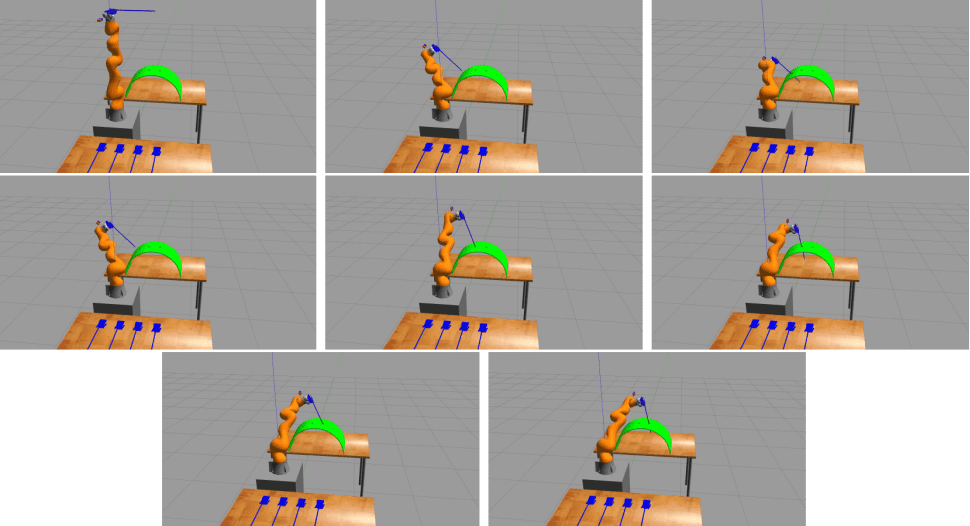
\includegraphics[width=\textwidth]{images/robot_planner2a}
\caption{Experiment 2a:}
\label{experiment-robot-planner2a}
\end{figure}
\end{center}

% Robot Planner 2a with RRTConnect
\begin{longtable}{|p{2cm}|c|p{2cm}|p{2cm}|p{2cm}|}
\hline
Robot Planner 2a           & \multicolumn{4}{c}{\textbf{RRTConnect}}                                                                                                 \vline \\
\hline
                          & \multicolumn{4}{c}{\textbf{Insertion \& Pivot trajectories}}                     \vline \\
\hline
Experiment                & Trocar1 insertion time & Execution status & Trocar1 retraction time & Execution status  \\
\hline
1	& 0.060728	& 1	& 2.875072	& 1 \\
2	& 0.070508	& 1	& 5.235667	& 1 \\
3	& 0.071487	& 1	& 5.239014	& 1 \\
4	& 0.059288	& 1	& 1.733352	& 1 \\
5	& 0.053619	& 1	& 3.376982	& 1 \\
6	& 0.062	& 1	& 5.389454	& 1 \\
7	& 0.084007	& 1	& -	& 0 \\
8	& 0.058306	& 1	& 5.254352	& 1 \\
9	& 0.046925	& 1	& 4.90185	& 1 \\
10	& 0.060491	& 1	& 5.073171	& 1 \\
\hline
\textbf{Average} & 	0.062736	& 1	& 4.342102	& 0.9 \\
\hline
\textbf{Standard deviation} & 	0.010348 &	- &	1.335526 & - \\
\hline
                          & \multicolumn{4}{c}{\textbf{Insertion \& Pivot trajectories}}                     \vline \\
\hline
Experiment                & Approach trocar2 time & Execution status & Trocar2 insertion time & Execution status  \\
\hline
1 & 2.67618	& 1	& 0.168283	& 1 \\
2 & 5.187283	& 1	& 0.179048	& 1 \\
3 & 0.050117	& 1	& 0.057194	& 1 \\
4 & 1.538822	& 1	& 0.184641	& 1 \\
5 & 1.62114	& 1	& 0.253224	& 1 \\
6 & 5.397757	& 1	& 0.268188	& 1 \\
7 & 5.379305	& 1	& 0.384924	& 1 \\
8 & 5.401832	& 1	& 0.193265	& 1 \\
9 & 2.845741	& 1	& 0.267069	& 1 \\
10  & 5.355111	& 1	& 0.250265	& 1 \\
\hline
\textbf{Average} & 3.545329	& 1	& 0.220610	& 1 \\
\hline
\textbf{Standard deviation} & 	2.038595 &	- &	0.086008 & - \\
\hline
                          & \multicolumn{4}{c}{\textbf{Insertion \& Pivot trajectories}}                     \vline \\
\hline
Experiment                & Trocar2 retraction time & Execution status & Approach trocar3 time & Execution status  \\
\hline
1 & 0.152233	& 1	& 0.214332	& 1 \\
2 & 0.321677	& 1	& 0.361712	& 1 \\
3 & 5.404121	& 1	& 5.271597	& 1 \\
4 & 0.147981	& 1	& 0.15915	& 1 \\
5 & 0.333447	& 1	& 0.298799	& 1 \\
6 & 0.246624	& 1	& 0.209347	& 1 \\
7 & 0.381983	& 1	& 0.473779	& 1 \\
8 & 0.219369	& 1	& 0.167211	& 1 \\
9 & 0.227563	& 1	& 0.297372	& 1 \\
10  & 5.149372	& 1	& 5.3578	& 1 \\
\hline
\textbf{Average} & 1.258437	& 1	& 1.281110	& 1 \\
\hline
\textbf{Standard deviation} & 	2.120018 &	- &	2.128103 & - \\
\hline
                          & \multicolumn{4}{c}{\textbf{Insertion \& Pivot trajectories}}                     \vline \\
\hline
Experiment                & Trocar3 insertion time & Execution status & Trocar3 retraction time & Execution status  \\
\hline
1 & 0.196175	& 1	& 0.855452	& 0 \\
2 & 0.412455	& 1	& 1.133213	& 0 \\
3 & 0.355923	& 1	& 0.814161	& 0 \\
4 & 0.194839	& 1	& 0.885119	& 0 \\
5 & 0.351561	& 1	& 0.364089	& 0 \\
6 & 0.355251	& 1	& 0.826636	& 0 \\
7 & 0.336123	& 1	& 0.30715	& 1 \\
8 & 0.147867	& 1	& 1.053035	& 0 \\
9 & 0.347956	& 0.6	& 0.80884	& 0.37  \\
10  & 0.28364	& 0.6	& 0.229825	& 1 \\
\hline
\textbf{Average} & 	0.298179	& 0.92 &	0.727752	& 0.237 \\
\hline
\textbf{Standard deviation} & 	0.088385 &	- &	0.314852 & - \\
\hline

\caption{Time results for robot planner 2a using the RRTConnect path planner algorithm. Planning time is the sum of solution time and path simplification time. Execution status is 
1 for success and 0 for failure. Parameters: tolerances: 0.0005, max planning time: 5 seconds, replanning: true, max planning attempts: 6. Experiments start from home position.}
\label{robot-planner2a-rrtconnect-data}
\end{longtable}

To overcome the reachability issue shown in Figure \ref{experiment-robot-planner2a}, the algorithm was repeated, but this time using a different simulation layout 
in Gazebo, in which the mounting dock is closer to the robot and in front of it. This new layout enables the robot to reach all mounting holes with ease and 
with sufficient dexterity, the robot is free to pivot around.

\begin{center}
\begin{figure}[!htb]
\centering
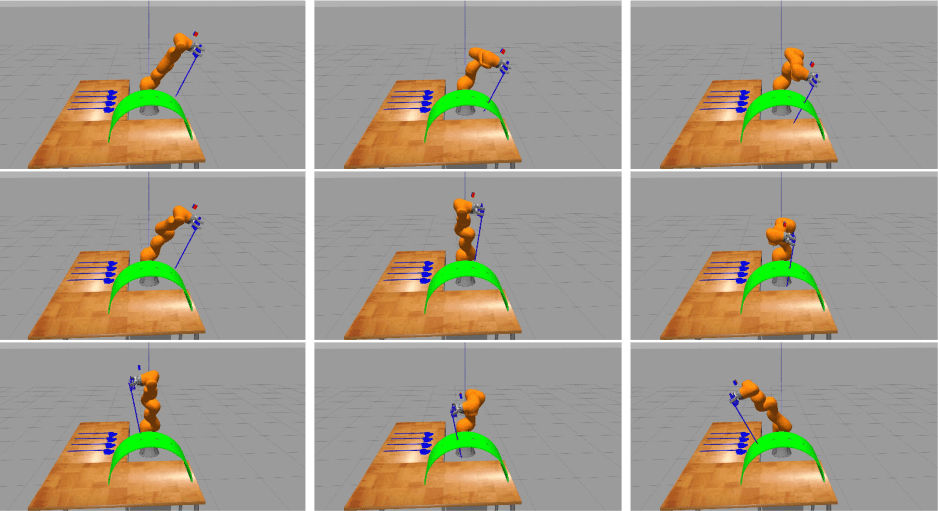
\includegraphics[width=\textwidth]{images/robot_planner2b}
\caption{Experiment 2b: Running robot planner 2b with a different table layout so that all target poses have improved reachability. Note that all trajectories shown in the screenshots are collision-free, 
because the robotic arm is in an elbow-up configuration, so that it avoids the collision between the 3rd link of the robot and the mounting dock (green object shown in simulation).}
\label{experiment-robot-planner2b}
\end{figure}
\end{center}

Observing the screenshots at figure \ref{experiment-robot-planner2b}, it is clear that the robot must always be in an elbow-up configuration in order to avoid collisions with the mounting dock. This constraint can be 
described either using the relative distance of the third link with the base or the relative angles of the third link's axis with respect to the axis of the base, as described with more detail in 
\ref{section-elbow-up-constraints}. The latter description with angles is easier to implement using the ROS MoveIt! framework,  but it would require to solve an extra inverse and forward kinematics problem targeting the third 
link, instead of the end-effector. To avoid these additional, computationally expensive calculations and simplify the experiments, instead of mathematically describing the constraint, 
some extra points were added in the trajectory. 
These points are usually close to the robot's axis and are such, that 
moveit will be forced to find a solution with an elbow-up configuration (because there will be no other solution satisfying the target point). Starting with an elbow-up configuration makes the path planner stick with that 
configuration for most of the path, because otherwise it would make a big jump in the joint state space which is not allowed from the parameters used in the experiments.

% Robot Planner 2b with RRTConnect
\begin{longtable}{|p{2cm}|c|p{2cm}|p{2cm}|p{2cm}|}
\hline
Robot Planner 2b           & \multicolumn{4}{c}{\textbf{RRTConnect}}                                                                                                 \vline \\
\hline
                          & \multicolumn{4}{c}{\textbf{Insertion \& Pivot trajectories}}                     \vline \\
\hline
Experiment                & Trocar1 insertion time & Execution status & Trocar1 retraction time & Execution status  \\
\hline
1	& 0.269901	& 1	& 0.355588	& 1 \\
2	& 0.220509	& 1	& 0.255968	& 1 \\
3	& 0.260483	& 1	& 5.28604	& 1 \\
4	& 0.267778	& 1	& 0.267796	& 1 \\
5	& 0.388487	& 1	& 5.321684	& 1 \\
6	& 0.316275	& 1	& 0.2088	& 1 \\
7	& 0.202614	& 1	& 0.14469	& 1 \\
8	& 0.289368	& 1	& 0.275917	& 1 \\
9	& 0.353631	& 1	& 0.353631	& 1 \\
10	& 0.185345	& 1	& 0.154755	& 1 \\
\hline
\textbf{Average} & 0.275439 &	1	& 1.262487	& 1 \\
\hline
\textbf{Standard deviation} & 	0.064555 &	- &	2.131175 & - \\
\hline
                          & \multicolumn{4}{c}{\textbf{Insertion \& Pivot trajectories}}                     \vline \\
\hline
Experiment                & Approach trocar2 time & Execution status & Trocar2 insertion time & Execution status  \\
\hline
1 & 0.322578	& 1	& 0.283497	& 1 \\
2 & 0.209871	& 1	& 0.410543	& 1 \\
3 & 5.099769	& 1	& 0.296228	& 1 \\
4 & 0.216997	& 1	& 0.342776	& 1 \\
5 & 5.328204	& 1	& 0.394472	& 1 \\
6 & 0.450936	& 1	& 0.249248	& 1 \\
7 & 0.336209	& 1	& 0.165375	& 1 \\
8 & 0.397699	& 1	& 0.202118	& 1 \\
9 & 0.235555	& 1	& 0.333129	& 1 \\
10  & 0.320059	& 1	& 0.343595	& 1 \\
\hline
\textbf{Average} & 1.291788	& 1	& 0.302098	& 1 \\
\hline
\textbf{Standard deviation} & 	2.069297 &	- &	0.079229 & - \\
\hline
                          & \multicolumn{4}{c}{\textbf{Insertion \& Pivot trajectories}}                     \vline \\
\hline
Experiment                & Trocar2 retraction time & Execution status & Approach trocar3 time & Execution status  \\
\hline
1 & 5.374646	& 1	& 5.451335	& 1 \\
2 & 0.452231	& 1	& 0.253669	& 1 \\
3 & 0.22638	& 1	& 0.383933	& 1 \\
4 & 5.371822	& 1	& 5.611649	& 1 \\
5 & 0.395787	& 1	& 0.309212	& 1 \\
6 & 5.15406	& 1	& 5.515007	& 1 \\
7 & 4.189377	& 1	& 5.570568	& 1 \\
8 & 5.167346	& 1	& 5.522056	& 1 \\
9 & 5.101735	& 1	& 5.452301	& 1 \\
10  & 5.273342	& 1	& 5.467273	& 1 \\
\hline
\textbf{Average} & 3.670673	& 1	& 3.953700	& 1 \\
\hline
\textbf{Standard deviation} & 	2.311081 &	- &	2.511216 & - \\
\hline
                          & \multicolumn{4}{c}{\textbf{Insertion \& Pivot trajectories}}                     \vline \\
\hline
Experiment                & Trocar3 insertion time & Execution status & Trocar3 retraction time & Execution status  \\
\hline
1 & 0.372382	& 1	& 5.34059	& 1 \\
2 & 0.280432	& 1	& 0.261765	& 1 \\
3 & 0.179581	& 1	& 0.187589	& 1 \\
4 & 0.121094	& 1	& 5.152808	& 1 \\
5 & 0.472468	& 1	& -	& 0 \\
6 & 0.251195	& 1	& 0.442282	& 0 \\
7 & 0.20647	& 1	& 0.318481	& 1 \\
8 & 0.178941	& 1	& 0.185758	& 1 \\
9 & 0.188906	& 1	& 0.222821	& 1 \\
10  & 0.165681	& 1	& 0.170876	& 1 \\
\hline
\textbf{Average} & 	0.241715  &	1 &	1.364774 &	0.8 \\
\hline
\textbf{Standard deviation} & 	0.107534 &	- &	2.202951 & - \\
\hline
\caption{Time results for robot planner 2b using the RRTConnect path planner algorithm and a different table layout from robot planner 2a. Planning time is the sum of solution time and path simplification time. Execution status is 
1 for success and 0 for failure. Parameters: tolerances: 0.0005, max planning time: 5 seconds, replanning: true, max planning attempts: 6. Experiments start from home position.}
\label{robot-planner2b-rrtconnect-data}
\end{longtable}


Due to the probabilistic nature of the motion planner (in these experiments the OMPL library is used with the RRTConnect path planning algorithm), the solutions 
to the path planning problem are not always the same and thus it is possible that the robot arm reaches a pose which is close to a singularity
\begin{center}
\begin{figure}[!htb]
\centering
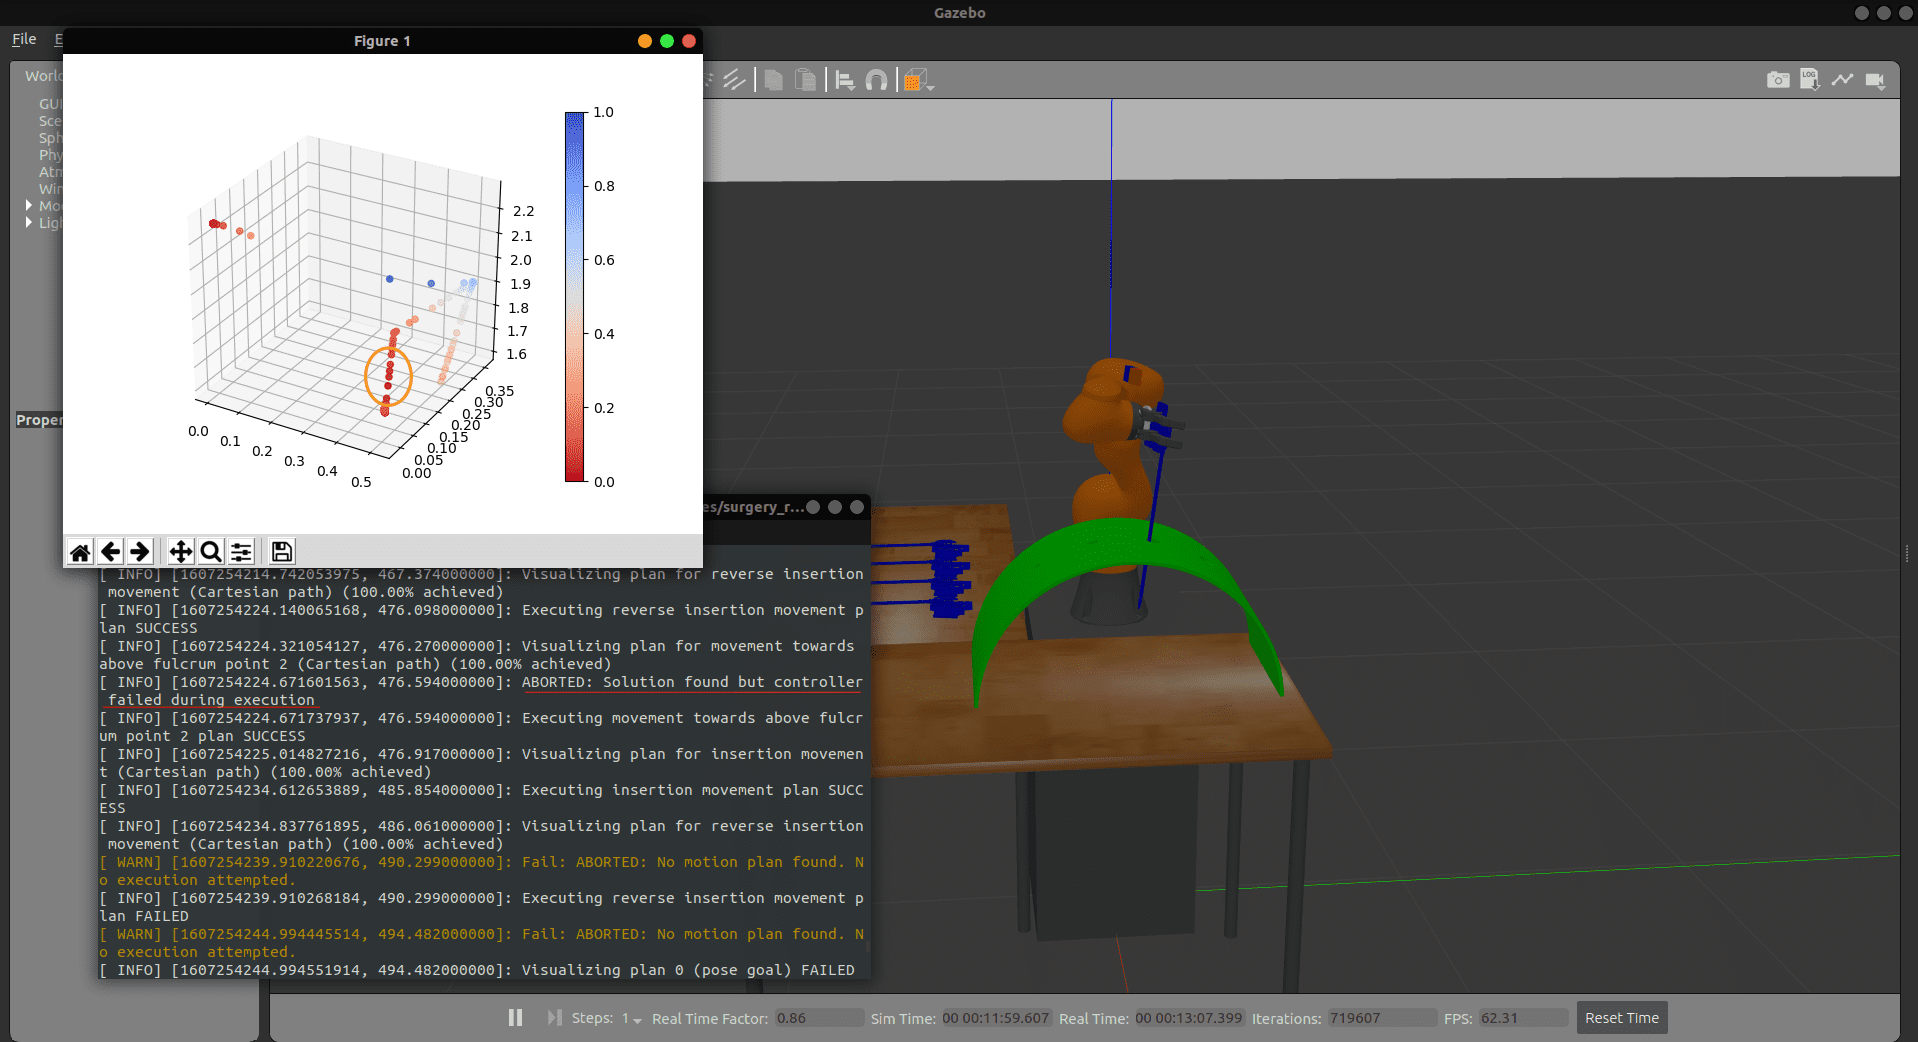
\includegraphics[width=0.9\textwidth]{images/robot_planner2b/singularity_failure.png}
\caption{Experiment 2b: Singularity failure}
\label{robot-planner2b-singularity-failure}
\end{figure}
\end{center}

Sometimes, when planning or executing a trajectory the robot may fail to complete the task because it has approached a singularity point. The points of singularity or of low dexterity are those points shown in the screenshot 
\ref{robot-planner2b-singularity-failure} which have red color. The color coding is calculated using the equation \ref{dexterity-measure}. The values of the Jacobian matrix are calculated at every kinematic state using 
a custom ROS node that subscribes to the robot's kinematic state (joints' angle positions, velocities, etc) and publishes the values of the Jacobian matrix as well as the forward kinematics solutions, to the 
/kinematic\_state topic (see figure \ref{kinematic-state-topic-graph}).

\begin{center}
\begin{figure}[!htb]
\centering

\includegraphics[width=\textwidth]{images/kinematic_state_topic_graph.png}
\caption{Custom kinematic state node that subscribes to the joint values and publishes forward kinematics solutions and the jacobian matrix values.}
\label{kinematic-state-topic-graph}
\end{figure}
\end{center}


\section{Robot Planner 3: Trajectory planning}

The goal of this third experiment is to design and test only some pivot trajectories. The pivot motions follow the equations described in 
\ref{section:pivot-motions}. The trajectories that were designed and tested in this group of experiments are the following:
\begin{itemize}
\item Line segment
\item Circle
\item Cubic spline
\item B-Spline
\item Quintic polynomial in joint space
\item Trapezoidal velocity profile in joint space
\item S-Curve velocity profile in joint space
\item Helix
\end{itemize}

\subsection{Line segment trajectories in task space}
\label{section:robot-planner3b}

The goal of this experiment is to generate a line segment trajectory inside the surgical
taskspace which will then be transformed via the fulcrum transformation to a trajectory that the robotic arm can execute. To define a line segment only 
2 points are needed, the coordinates of the start and those of the end of the line segment. An other, way of defining a line segment trajectory, 
is by passing as parameters the coordinates of the start point and a vector attached to that point, whose and points to the end point. The second definition 
of the line segment can be very useful in cases where the direction of the line is needed.

\begin{center}
\begin{figure}[!htb]
\centering
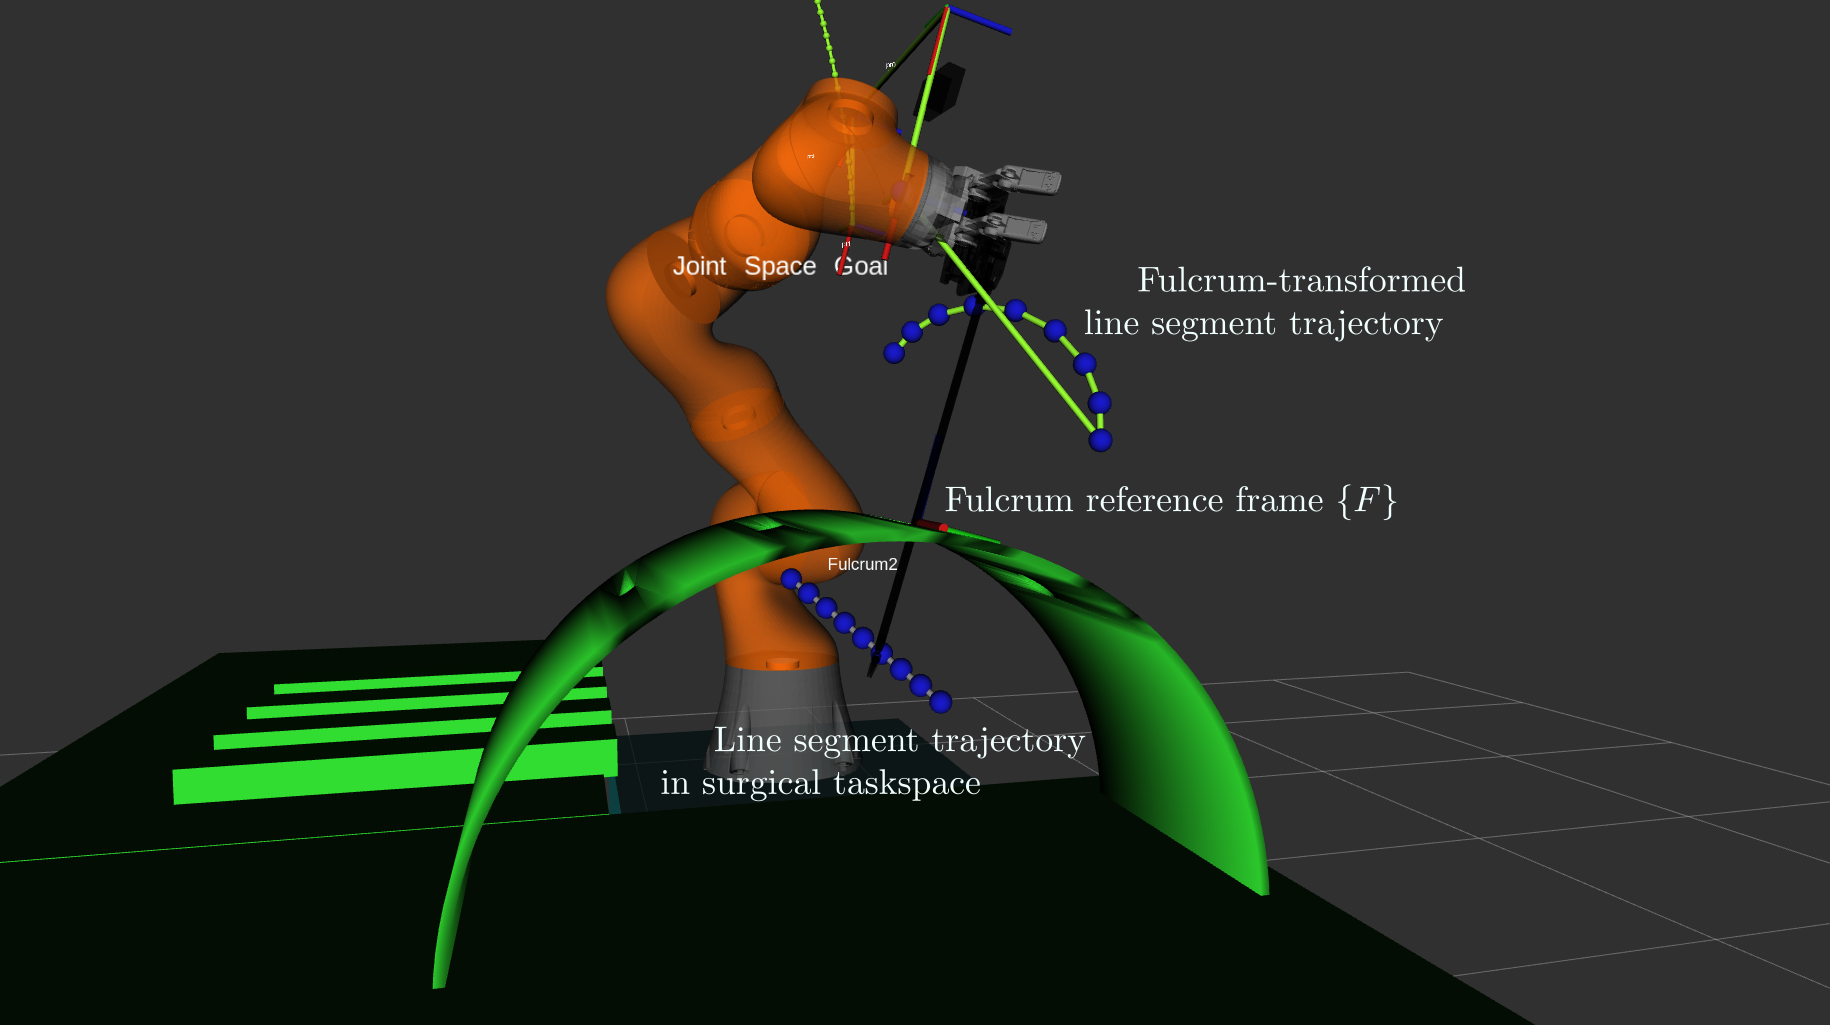
\includegraphics[width=\textwidth]{images/robot_planner3/3b_line_seg.png}
\caption{Experiment 3b: Create the line segment trajectory inside the surgical site (below the green mounting dock) and transform it via the fulcrum transformation to a trajectory for the robot's TCP.
(a) Preparatory path to achieve elbow-up pose, (b) transformed line segment trajectory for the end-effector to follow, (c) transformed line segment trajectory with respect to the tool base frame (there is an offset from the 
end-effector see \ref{section:eef-tool-tip-transformations}), (d) fulcrum reference frame 2 $\lbrace F_2 \rbrace$, (e) line segment trajectory in surgical taskspace, (f) line of the axis along the length of the surgical tool, 
which is used to calculated the distance error (RCM deviation)}
\label{robot-planner3b-line-seg}
\end{figure}
\end{center}

\begin{center}
\begin{figure}[!htb]
\centering
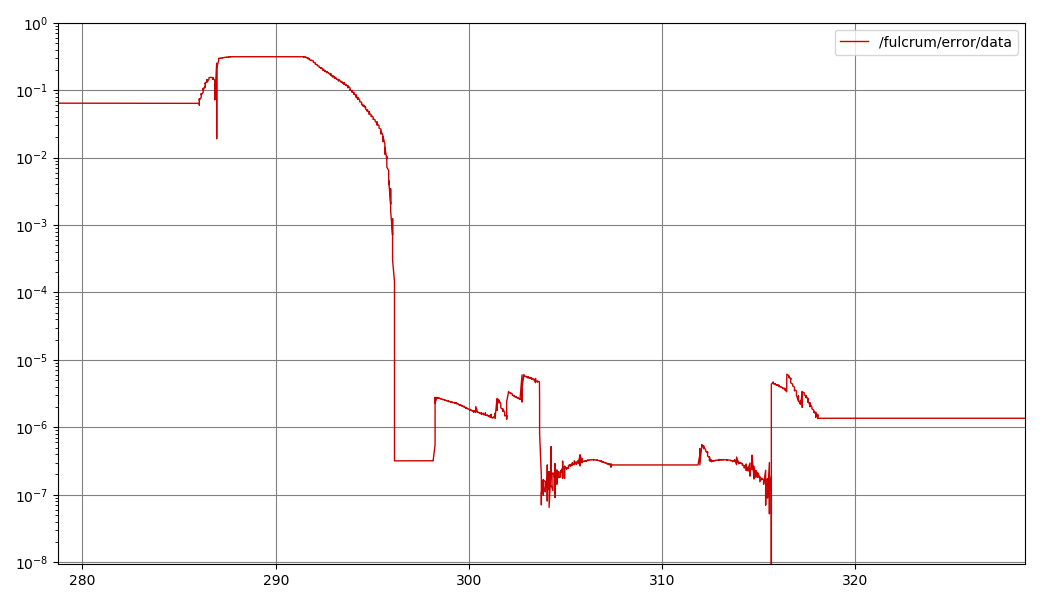
\includegraphics[width=\textwidth]{images/robot_planner3/robot_planner3b_error.png}
\caption{Experiment 3b: RCM error diagram from home position to line and reverse-line segment trajectories.}
\label{robot-planner3b-line-seg-rcm-errors}
\end{figure}
\end{center}

In the diagram \ref{robot-planner3b-line-seg-rcm-errors} one can see the RCM error values with respect to time. The x-axis shows the ROS time in seconds and the y-axis the RCM error in logarithmic scale. The robot starts from 
the home position where the rcm error is bigger, then approaches the fulcrum point, 
where the error decreases and then it executes the line segment pivot trajectory where the error is bounded in the magnitude of less than a micrometer $10^{-6}m$ then stays constant, then changes again during the execution of 
the reverse line-segment trajectory and then finally it stays constant while the robot stays still in the initial insertion position. The RCM error while the robot is inserted but still and the error while the robot executes 
a pivot trajectory are studied separately.

\begin{center}
\begin{figure}[!htb]
\centering
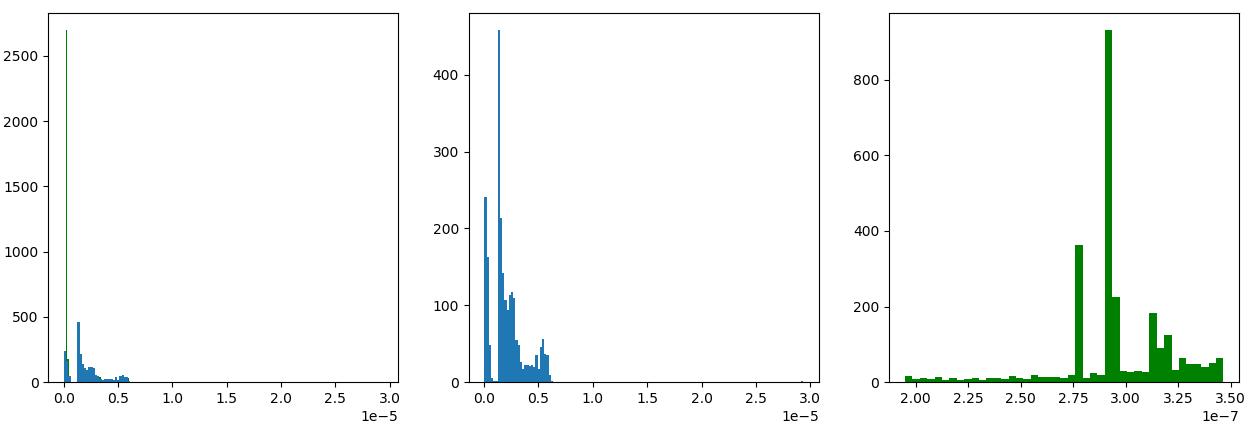
\includegraphics[width=\textwidth]{images/robot_planner3/robot_planner3b-error_distributions.png}
\caption{Experiment 3b: RCM error distributions, measurements from 10 iterations of the same experiment. From left to right: distribution of all measurements, distribution of measurements while the robot was pivoting, 
distribution of measurements while the robot was inserted but still.}
\label{robot-planner3b-line-seg-rcm-error-distributions}
\end{figure}
\end{center}

\begin{table}[!htb]
\centering
\begin{tabular}{ |c|c|c|c| } 
\hline
 & Average [m] & Standard Deviation [m] & sample size \\
 & (accuracy) & (repeatability) & \\
\hline
\textbf{while pivoting} & $2.112649 \cdot 10^{-6}$ & $1.609277 \cdot 10^{-6}$ & 2309 \\
\hline
\textbf{while inserted and still} & $2.948652 \cdot 10^{-7}$ & $2.948652 \cdot 10^{-7}$ & 2696 \\
\hline
\end{tabular}
\caption{Accuracy and repeatability of the line segment experiment, calculated using measurements from 10 iterations of the same experiment}
\end{table}

\begin{center}
\begin{figure}[!htb]
\centering
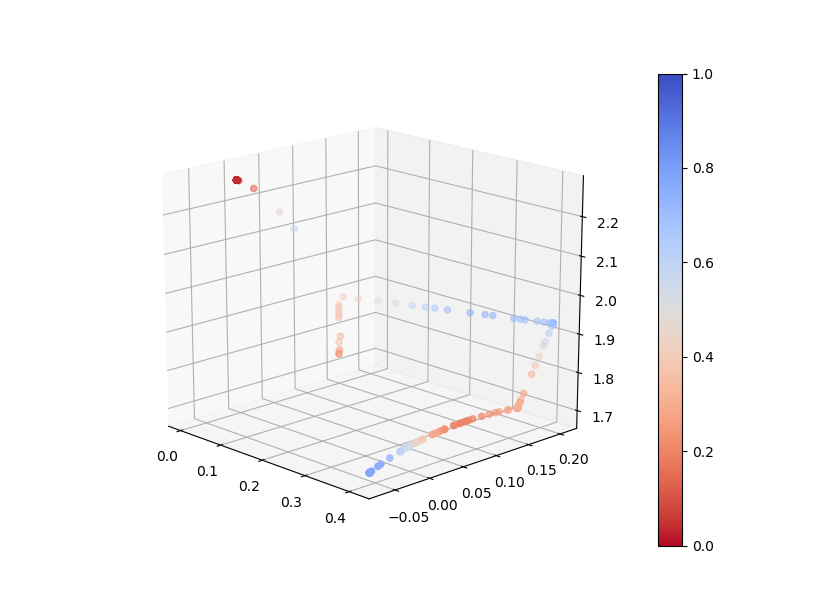
\includegraphics[width=0.49\textwidth]{images/robot_planner3/robot_planner3b_manip1.png}
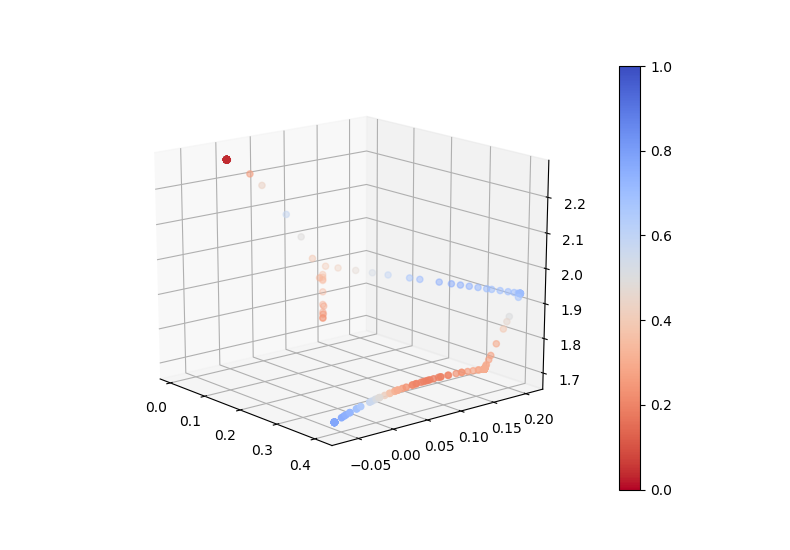
\includegraphics[width=0.49\textwidth]{images/robot_planner3/robot_planner3b_manip2.png}
\caption{Experiment 3b: Manipulability plots of the whole trajectory the robot executed during 2 iterations of the same experiment}
\label{robot-planner3b-line-seg-manipulability-plots}
\end{figure}
\end{center}

Note that although this type of trajectory is trivial in robot planner, this specific line segment trajectory should not be confused with ROS MoveIt line segment trajectories. The line-segment studied in this experiment 
is linear when defined in the surgical taskpsace, but it is highly non-linear when transformed via the fulcrum transformation and it has a curved shape. The only exceptions to this transformation is for line segments that 
lie on the direction defined by the radius unit vector $\mathbf{\hat{r}}$ of the spherical coordinate system of the Fulcrum reference frame, or equivalently the points $A,B$ defining the line-segment and the origin $O$ 
of the reference frame, must be collinear. These exceptions can also be planned by the MoveIt framework and are also known 
as and referenced throughout this thesis, as insertion movements. Let $\overrightarrow{AB}$ be the vector representing the line segment, then for the points $A, B$ the following must hold, in order for the line segment to be 
invariant under the fulcrum transformation in terms of shape (i.e. the line to remain a line).
\begin{equation}
\overrightarrow{AB} = \overrightarrow{OB} - \overrightarrow{OA}
\end{equation} 
and
\begin{equation}
\overrightarrow{OB} = r \overrightarrow{OA}, \quad r \in \mathbb{R}
\end{equation}

\begin{center}
\begin{figure}[!htb]
\centering
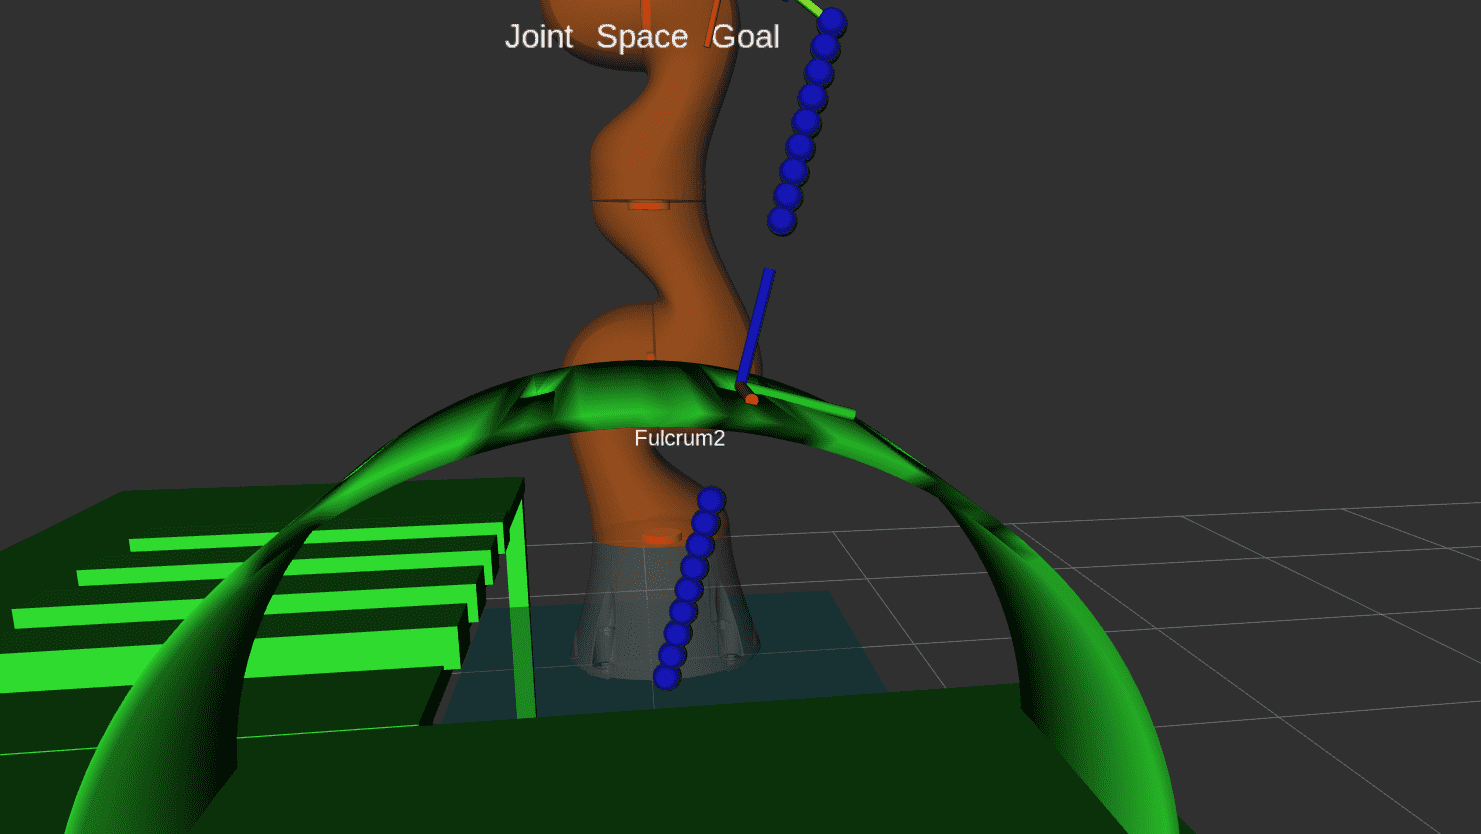
\includegraphics[width=\textwidth]{images/robot_planner3/3b_line_seg_invariant.png}
\caption{Experiment 3b: Line segment trajectory that is invariant under the fulcrum transformation, in terms of shape (the line remains a line).}
\label{robot-planner3b-line-seg}
\end{figure}
\end{center}

% Robot Planner 3b with RRTConnect
\begin{longtable}{|p{0.16\textwidth}|p{0.16\textwidth}|p{0.16\textwidth}|p{0.16\textwidth}|p{0.16\textwidth}|}
\hline
Robot Planner 3b          & \multicolumn{4}{c}{Approach and \textbf{line segment pivot} trajectories with \textbf{RRTConnect}}                                                                                                 \vline \\
\hline
                          & \multicolumn{4}{c}{\textbf{elbow-up preparatory path}}                     \vline \\
\hline
Experiment                & Elbow-up Start pose planning time (sec) & Execution status & Elbow-up preparation path planning time (sec) & Execution status  \\
\hline
1 & 0.221091 & 1 & 0.074075 & 1 \\
2 & 0.19466 & 1 & 0.194823 & 1 \\
3 & 0.268828 & 1 & 0.073928 & 1 \\
4 & 0.154783 & 1 & 0.049908 & 1 \\
5 & 0.110496 & 1 & 0.104181 & 1 \\
6 & 0.155316 & 1 & 0.061127 & 1 \\
7 & 0.140189 & 1 & 0.048735 & 1 \\
8 & 0.166412 & 1 & 0.261208 & 1 \\
9 & 0.121243 & 1 & 0.247453 & 1 \\
10 & 0.209206 & 1 & 0.054966 & 1 \\
\hline
\textbf{Average} & 0.174222 & 1 & 0.117040	& 1 \\
\hline
\textbf{Standard deviation} & 	0.049002 &	- &	0.084238 & - \\
\hline
                          & \multicolumn{4}{c}{\textbf{Approach \& Insertion}}                     \vline \\
\hline
Experiment                & Approach fulcrum 2 path planning time (sec) & Execution status & Insertion path planning time (sec) & Execution status  \\
\hline
1 & 0.067982 & 1 & 0.30244 & 1 \\
2 & 0.345301 & 1 & 0.325638 & 1 \\
3 & 0.112407 & 1 & 0.173074 & 1 \\
4 & 0.054112 & 1 & 0.194001 & 1 \\
5 & 0.117048 & 1 & 0.23512 & 1 \\
6 & 0.055864 & 1 & 0.284625 & 1 \\
7 & 0.07501 & 1 & 0.231642 & 1 \\
8 & 0.170249 & 1 & 0.105259 & 1 \\
9 & 0.102762 & 1 & 0.374426 & 1 \\
10 & 0.064243 & 1 & 0.269333 & 1 \\
\hline
\textbf{Average} & 0.116498 &	1 &	0.249556 &	1 \\
\hline
\textbf{Standard deviation} & 	0.088078 &	- &	0.078941 & - \\
\hline
                          & \multicolumn{4}{c}{\textbf{Line segment pivot trajectories}}                     \vline \\
\hline
Experiment                & Line segment path planning time (sec) & Execution status & Reverse line segment path planning time (sec) & Execution status  \\
\hline
1 & 5.326128 & 1 & 5.486623 & 1 \\
2 & 0.479823 & 1 & 5.279854 & 1 \\
3 & 0.288405 & 1 & - & 0 \\
4 & 0.295343 & 1 & - & 0 \\
5 & 0.225066 & 1 & 5.445483 & 1 \\
6 & 5.132968 & 1 & - & 0 \\
7 & 0.300322 & 1 & 5.285311 & 1 \\
8 & 5.484813 & 1 & 5.403696 & 1 \\
9 & 0.297406 & 1 & 5.309383 & 1 \\
10 & 0.259739 & 1 & 5.285902 & 1 \\
\hline
\textbf{Average} & 1.809001 &	1 &	5.356607 &	0.7 \\
\hline
\textbf{Standard deviation} & 	2.421448 &	- &	0.086818 & - \\
\hline
\caption{Time results for robot planner 1 using the RRTConnect path planner algorithm. Planning time is the sum of solution time and path simplification time. Execution status is 
1 for success and 0 for failure. Parameters: tolerances: 0.000005, max planning time: 5 seconds, replanning: true, max planning attempts: 6. Experiments start from home position.}
\label{robot-planner3b-rrtconnect-data}
\end{longtable}


\subsection{Circular trajectories in task space}

The goal of this experiment is to generate a circular trajectory inside the surgical taskspace which will then be transformed via the fulcrum transformation 
to a trajectory that the robotic arm can execute. To define a circular trajectory in the taskspace, two parameters are required: the $(x,y,z)$ coordinates of the 
circle's center and it's radius $r$.\\ 

\begin{center}
\begin{figure}[!htb]
\centering
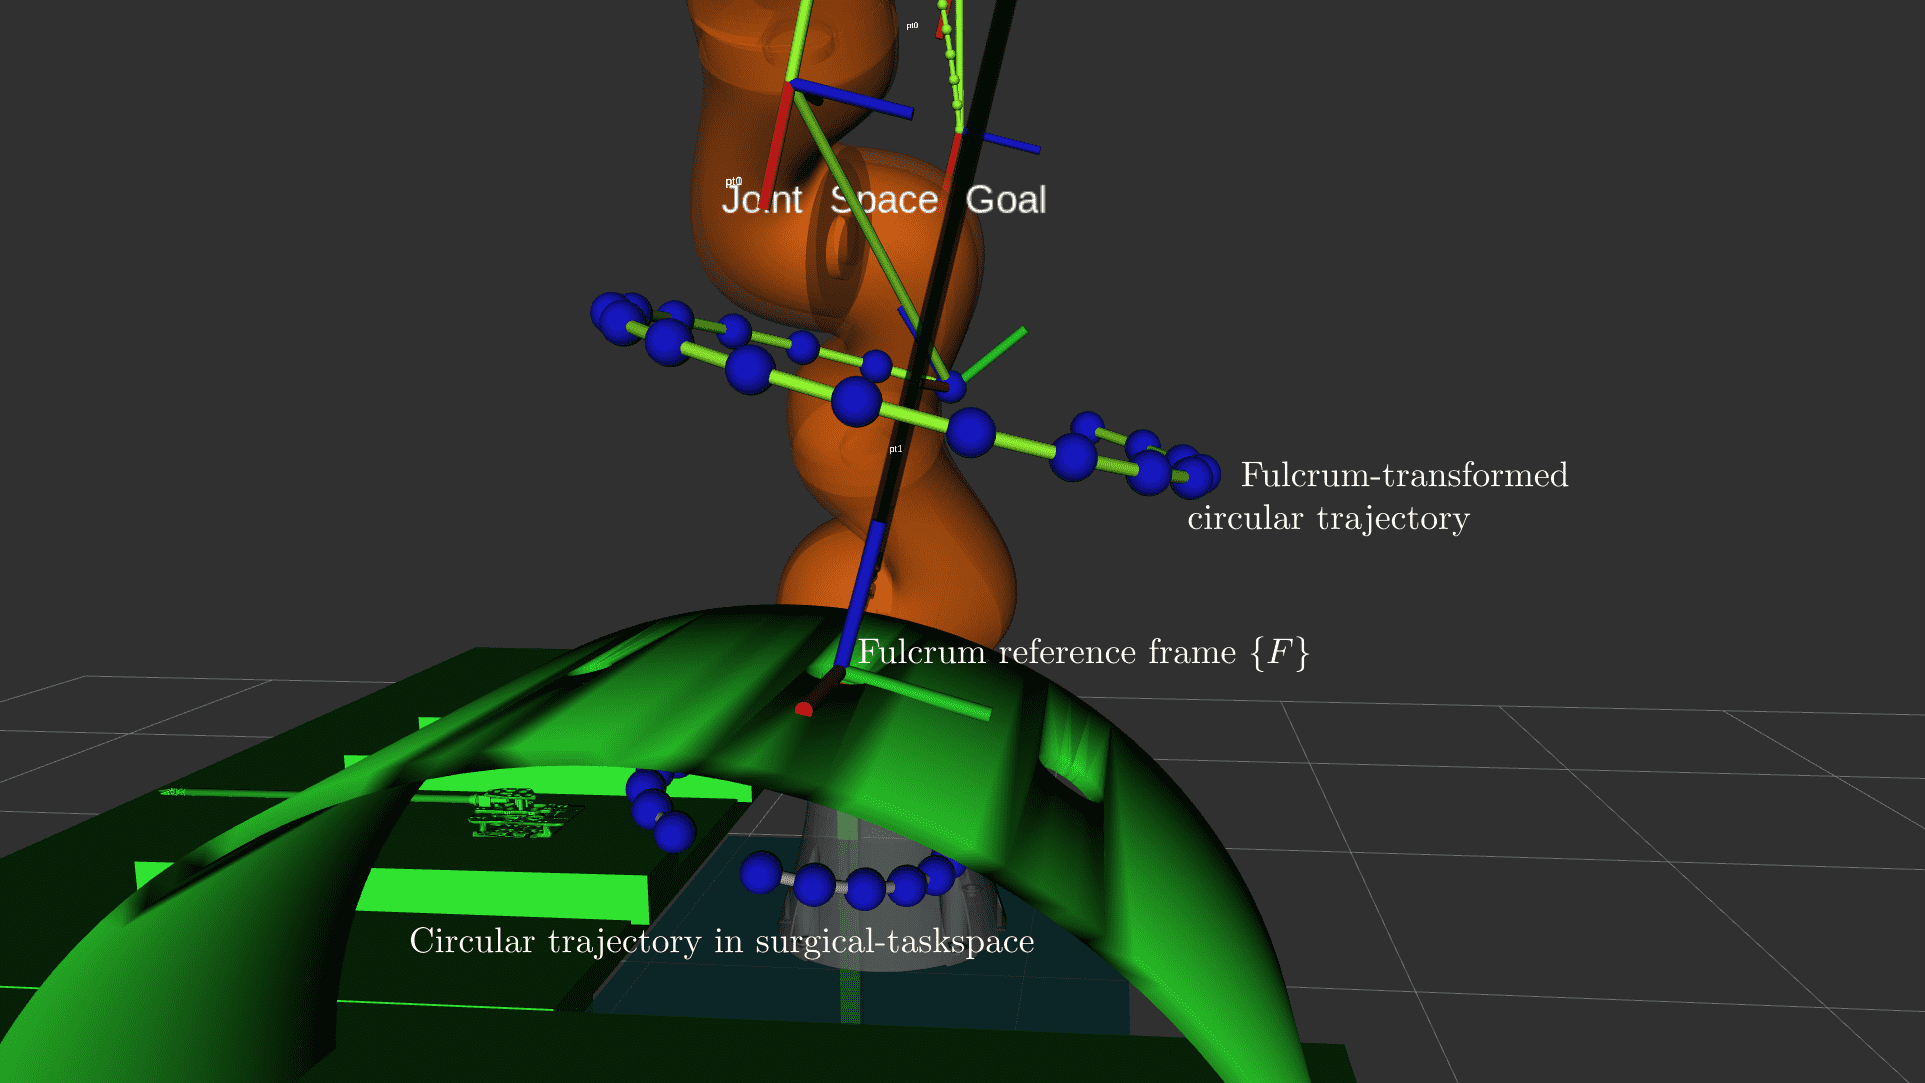
\includegraphics[width=\textwidth]{images/robot_planner3/3a_circle.png}
\caption{Experiment 3a: Create circular trajectory inside the surgical site (below the green mounting dock) and transform it via the fulcrum transformation to a trajectory for the robot's TCP.}
\label{robot-planner3a-circle}
\end{figure}
\end{center}

\begin{center}
\begin{figure}[!htb]
\centering
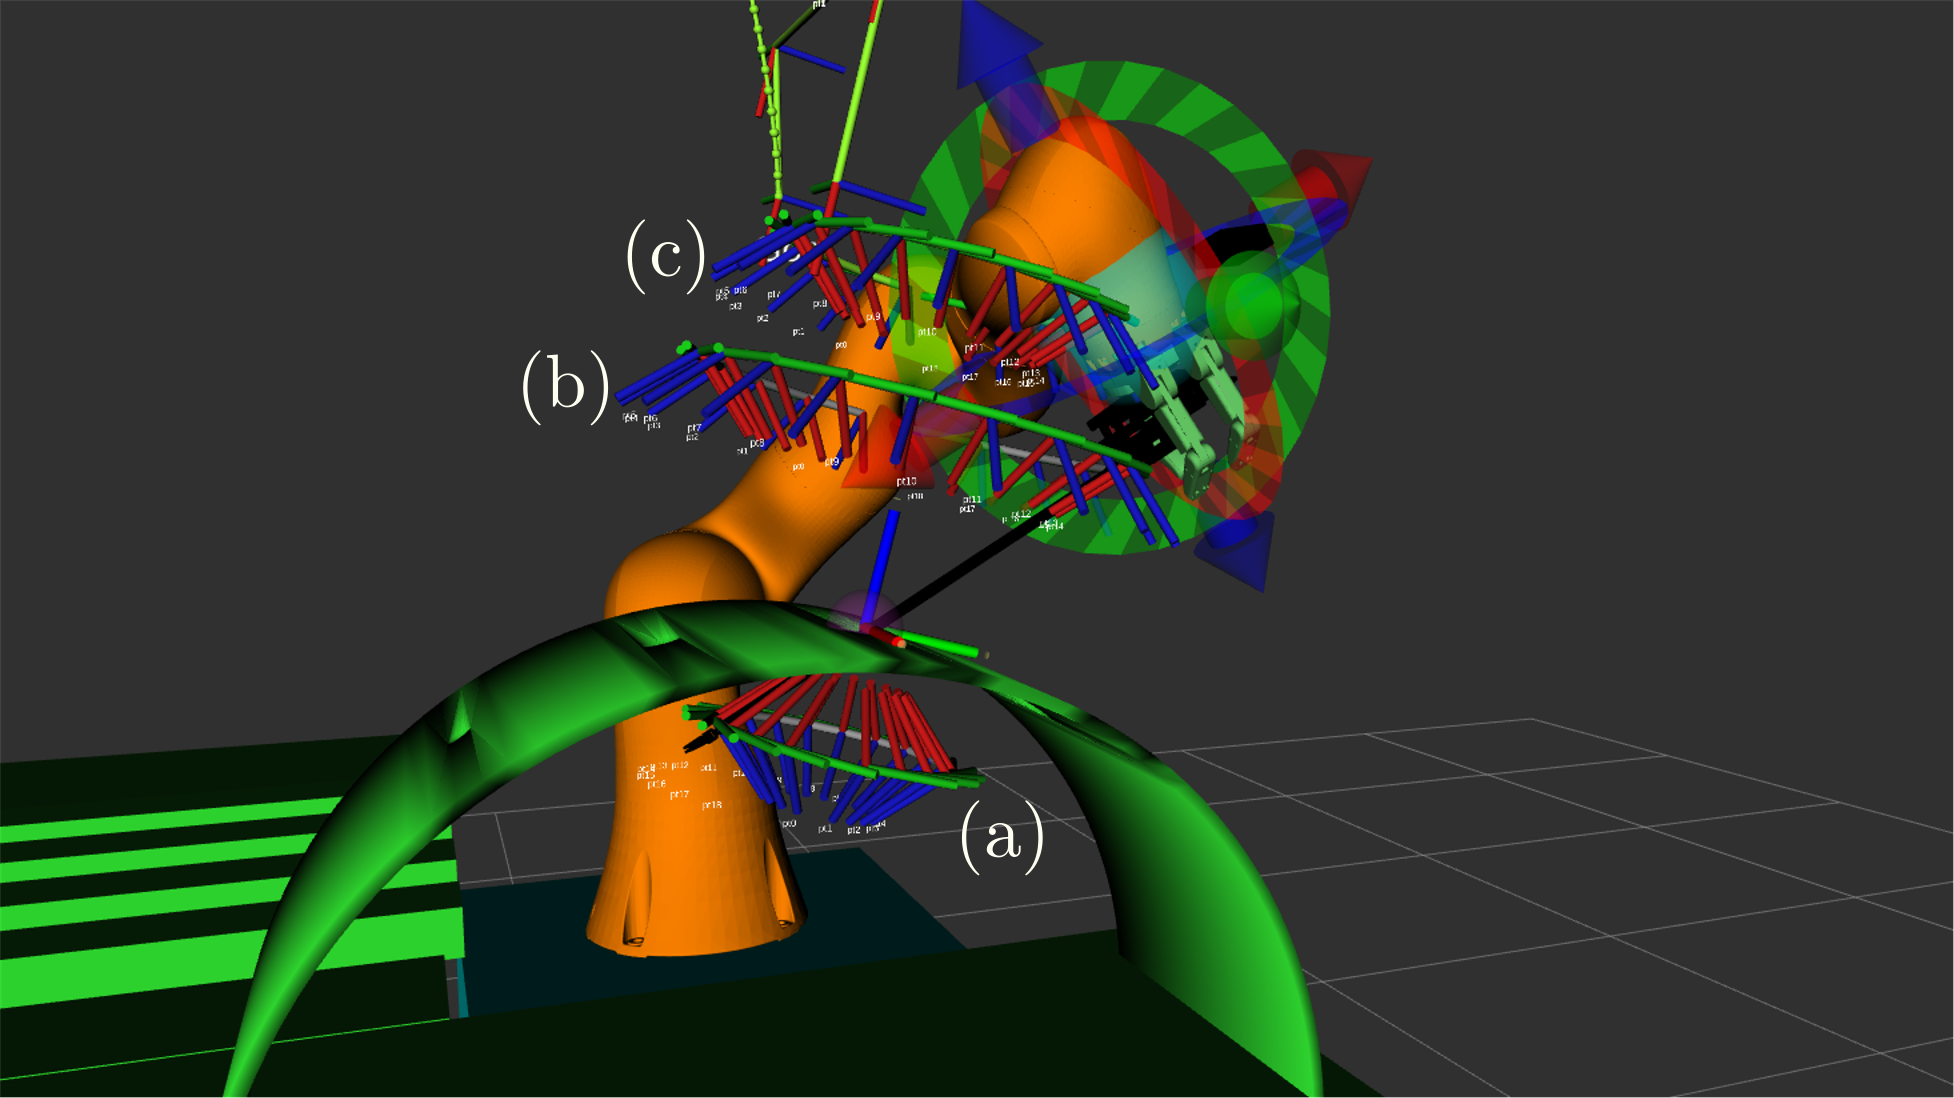
\includegraphics[width=\textwidth]{images/robot_planner3/3a_circle_details.png}
\caption{Experiment 3a: A more detailed view of the circular trajectories. (a) the original circular trajectory designed inside the surgical taskspace, (b) the transformed trajectory that the base of the surgical tool will
 follow, (c) the actual transformed trajectory that the robot's end-effector will follow}
\label{robot-planner3a-circle-details}
\end{figure}
\end{center}

Note that in this experiment (see screenshot \ref{robot-planner3a-circle}), the trivial case is examined where the circle is parallel to the $xy$ plane of the fulcrum's 
coordinate system. That is because the parametric definition if the circle, can be easily expressed when in a standard plane of the coordinate system i.e. $xy, xz$ 
or $yz$ planes and not in an arbitrary orientation.


\subsection{Cubic Spline trajectories in task space}

The goal of this experiment is to generate a cubic spline trajectory inside the surgical
taskspace which will then be transformed via the fulcrum transformation to a trajectory that the robotic arm can execute.

\begin{center}
\begin{figure}[!htb]
\centering
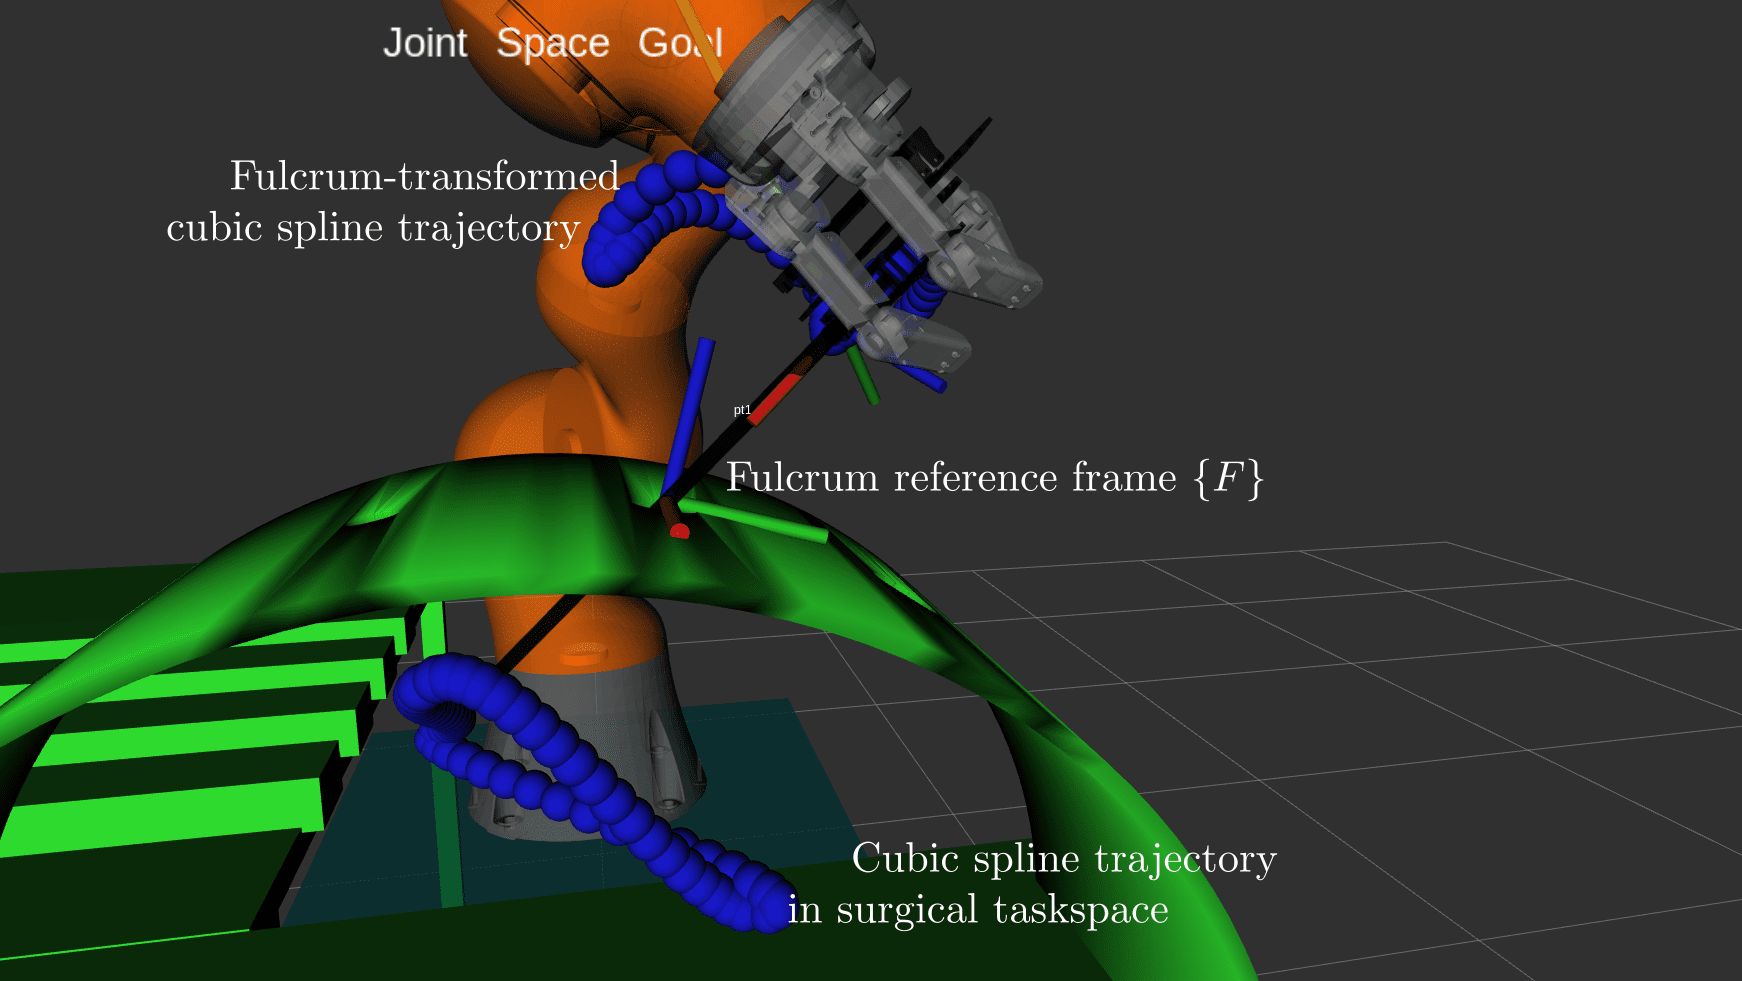
\includegraphics[width=\textwidth]{images/robot_planner3/3c_cubic_spline.png}
\caption{Experiment 3c: Create the cubic spline trajectory inside the surgical site (below the green mounting dock) and transform it via the fulcrum transformation to a trajectory for the robot's TCP.}
\label{robot-planner3c-cubic-spline}
\end{figure}
\end{center}

As seen on the screenshot \ref{robot-planner3c-cubic-spline}, for the surgical task there are 4 four points that were selected to create 3 cubic splines. The points that define the trajectory were:
\[
\begin{aligned}
\mathbf{x}_1 ={}& [-0.1, -0.1, -0.2] \\
\mathbf{x}_2 ={}& [0.1, -0.1, -0.1] \\
\mathbf{x}_3 ={}& [0.1, 0.1, -0.2] \\
\mathbf{x}_4 ={}& [-0.1, -0.1, -0.2] = \mathbf{x}_1
\end{aligned}
\]

and a constant derivative for all points of $\mathbf{x}_d = [0.1, 0.1, 0.1]$. Note that this derivative describes the shape and smoothness at the points that connect 
2 consecutive splines. These derivatives may not necessarily express a velocity in the cartesian space. That is because this derivative is calculated with respect 
to the path variable $s$. The time derivative of the trajectory would be calculated using the chain rule:

\begin{equation}
\begin{aligned}
\mathbf{\dot{x}} ={}& \frac{d\mathbf{x}}{dt}  \\
	={}& \frac{d\mathbf{x}(s)}{dt} = \frac{d\mathbf{x}(s(t))}{dt}   \\
    ={}& \frac{d\mathbf{x}}{ds} \cdot \frac{ds}{dt} \\
    ={}& \mathbf{x}_d \cdot \frac{ds}{dt}
\end{aligned}
\end{equation}


\subsection{B-Spline trajectories in task space}

\begin{center}
\begin{figure}[!htb]
\centering
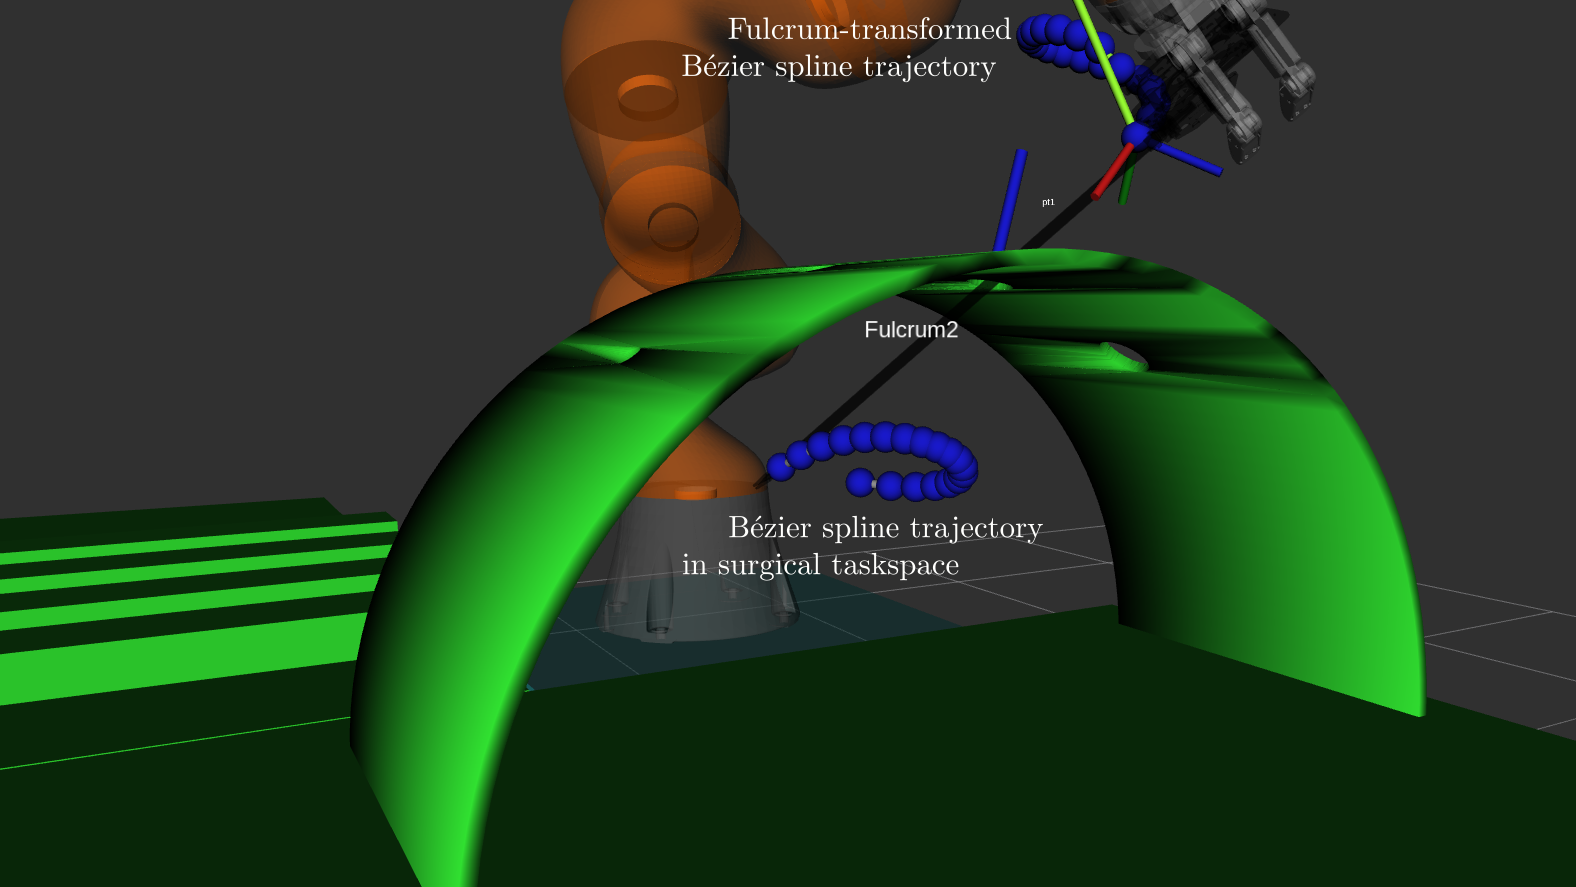
\includegraphics[width=\textwidth]{images/robot_planner3/3d_bezier_spline.png}
\caption{Experiment 3d: Create the B-spline trajectory inside the surgical site (below the green mounting dock) and transform it via the fulcrum transformation to a trajectory for the robot's TCP.}
\label{robot-planner3d-bezier-spline}
\end{figure}
\end{center}


\subsection{Polynomial trajectories in joint space}
\label{section:9-2-polynomial-traj}

The goal of this experiment is to generate a trajectory in joint space using a polynomial of 5th degree (see \ref{section-polynomials-5}). To generate this trajectory, at least 2 points are needed in the cartesian 
space. For each of these points the inverse kinematics problem is solved. The joint values of the first point are used as the start points of the trajectory and the joint values of the second point are used as the end points.
The velocities and accelerations are chosen to be zero for both start and end positions. The poses of the 2 points that were used as input to the 2 IK problems are

\[
T_A = 
\begin{bmatrix}
  &            &   & 0.1 \\
  & \mathbf{R_{rpy}} &   & 0.1 \\
  &            &   & 1.95 \\
0 &     0      & 0 & 1 \\
\end{bmatrix}
\]
\[
T_B = 
\begin{bmatrix}
  &            &   & 0.4 \\
  & \mathbf{R_{rpy}} &   & 0.1 \\
  &            &   & 1.95 \\
0 &     0      & 0 & 1 \\
\end{bmatrix}
\]
where 
\[
\mathbf{R_{rpy}} = \mathbf{Rot}(\mathbf{\hat{z}}, 2.952052) \cdot \mathbf{Rot}(\mathbf{\hat{y}}, 1.311528) \cdot \mathbf{Rot}(\mathbf{\hat{x}}, -1.750799)
\]

and the solutions chosen for each point are

\[
\mathbf{q_A} =
\begin{bmatrix}
1.148534 \\
-0.583084 \\ 
-0.212395 \\ 
-1.430756 \\
0.609015 \\ 
1.168518 \\ 
-0.523555 \\
\end{bmatrix}
\quad \textrm{and} \quad
\mathbf{q_B} = 
\begin{bmatrix}
2.293053 \\ 
-0.277892 \\
-1.795364 \\ 
-0.941923 \\ 
0.876039 \\
1.451593 \\
-0.916277 \\
\end{bmatrix}
\]

\begin{center}
\begin{figure}[H]
\centering
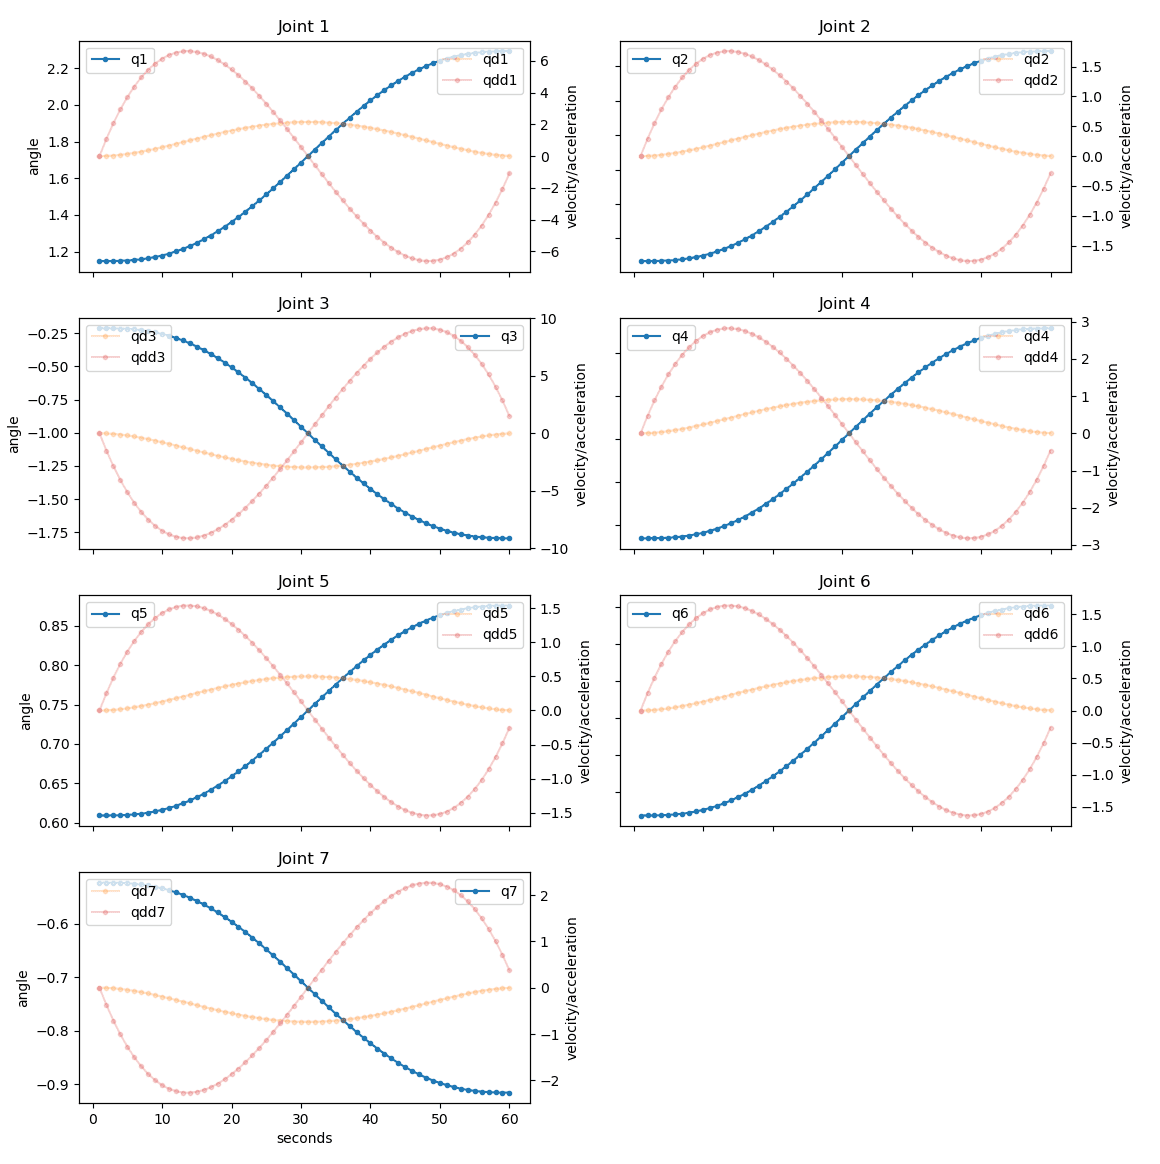
\includegraphics[width=\textwidth]{images/robot_planner3/3e_joint_polynomial.png}
\caption{Experiment 3e: Polynomial trajectories of 5th degree for each of the 7 joints. The trajectory is computed at 60 sampling points.}
\label{robot-planner3e-joint-polynomial}
\end{figure}
\end{center}


\subsection{Trajectories in joint space with trapezoidal velocity profile}

The goal of this experiment is to generate a trajectory in joint space using a trapezoidal velocity profile. The start and end points as well as the inverse kinematics solutions for these points are the same as those 
in \ref{section:9-2-polynomial-traj}.

\begin{center}
\begin{figure}[H]
\centering
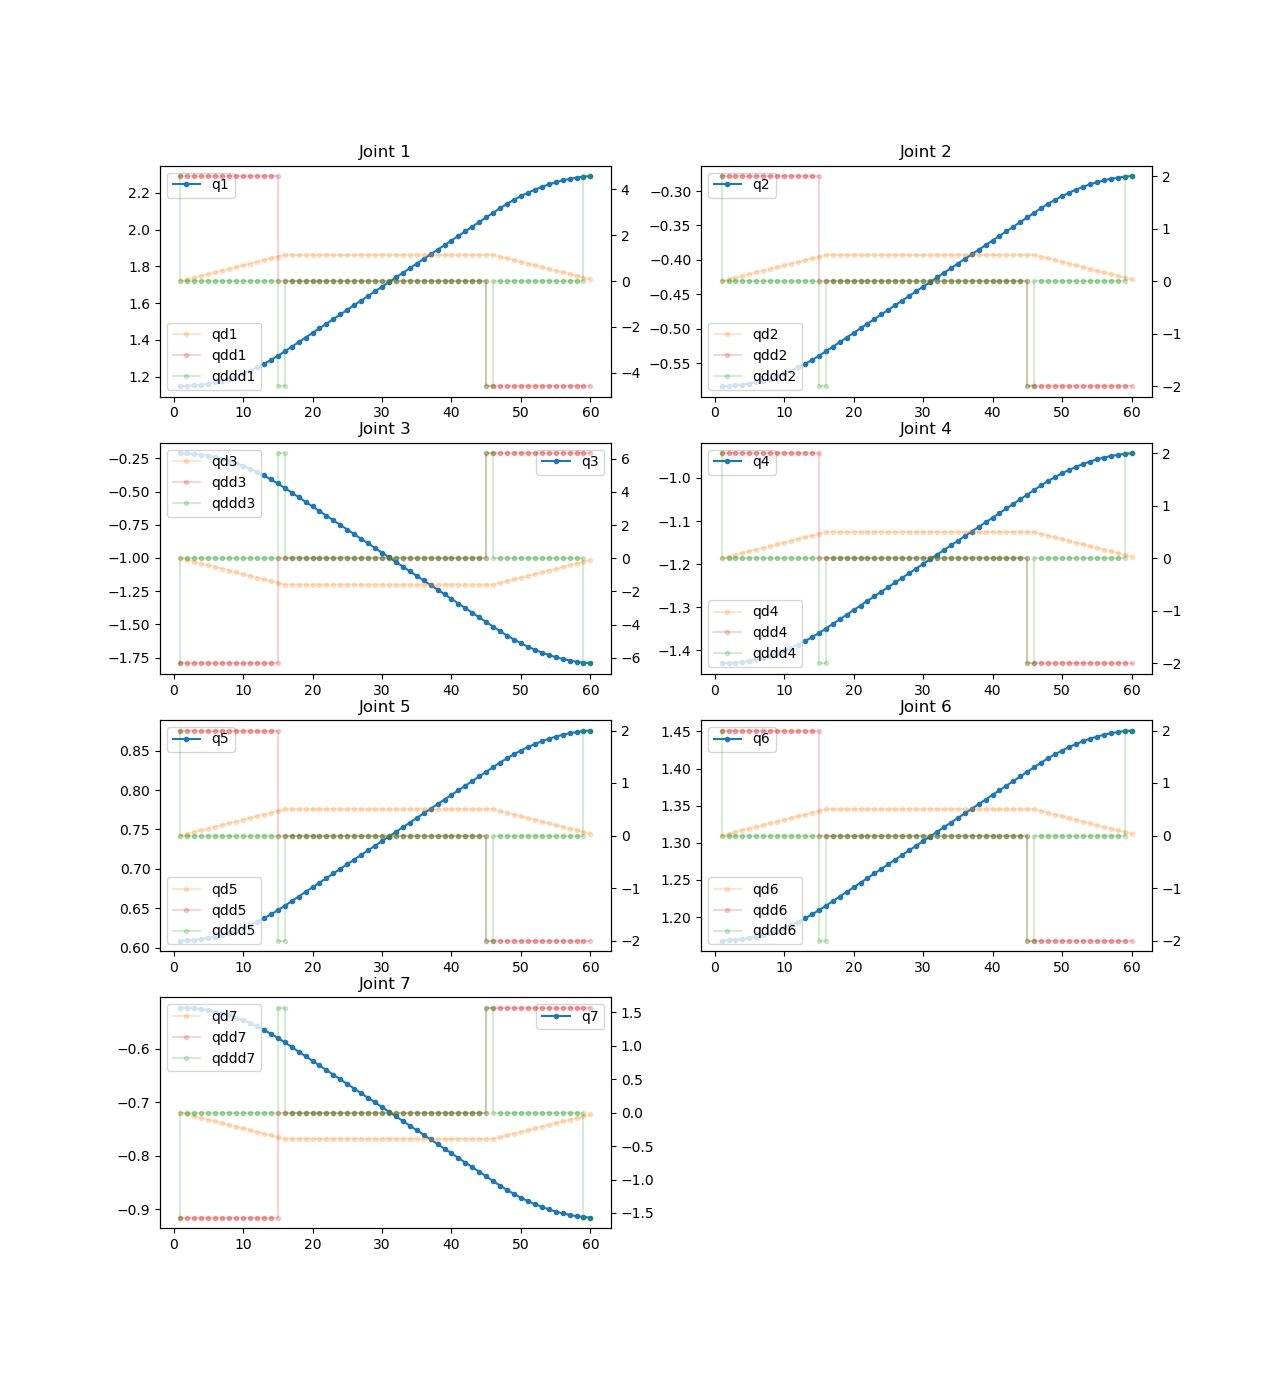
\includegraphics[width=\textwidth]{images/robot_planner3/3f_trapezoid1.png}
\caption{Experiment 3f: Trajectory using a trapezoid velocity profile. The time constant (also known as blend time) is $τ = 15$ seconds and the total trajectory duration is 60 seconds. The trajectory is computed at 60 sampling points.}
\label{robot-planner3f-joint-trapezoid1}
\end{figure}
\end{center}

\begin{center}
\begin{figure}[H]
\centering
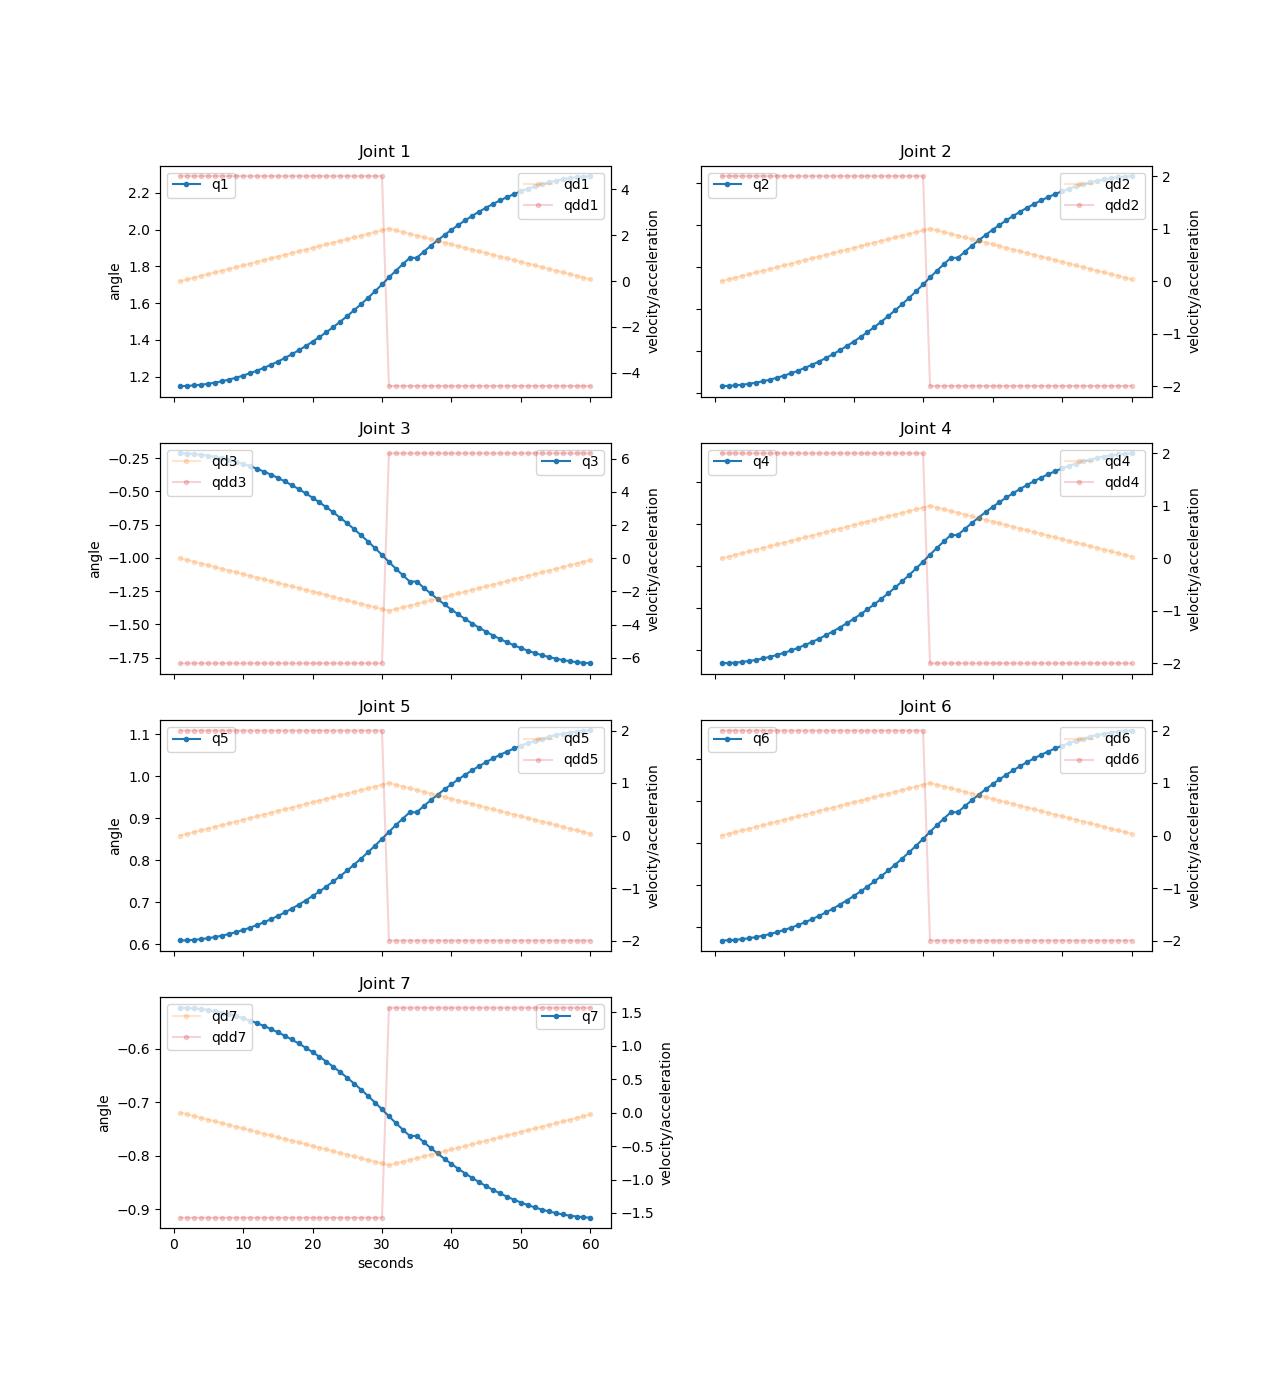
\includegraphics[width=\textwidth]{images/robot_planner3/3f_trapezoid2.png}
\caption{Experiment 3f: Trajectory using a trapezoid velocity profile. The time constant (also known as blend time) is $τ = 30$ seconds and the total trajectory duration is 60 seconds. Note that 
the blend time is chosen as half of the total duration which has as a result the linear segment (constant velocity) to disappear and create a "bang-bang" trajectory. In control theory, a "bang-bang" controller, 
is a controller that switches abruptly between two states. The trajectory is computed at 60 sampling points.}
\label{robot-planner3f-joint-trapezoid2}
\end{figure}
\end{center}


\subsection{Trajectories in joint space with s-curve velocity profile}

The goal of this experiment is to generate a trajectory in joint space using a smooth s-curve velocity profile. The start and end points as well as the inverse kinematics solutions for these points are the same as those 
in \ref{section:9-2-polynomial-traj}.

\begin{center}
\begin{figure}[H]
\centering
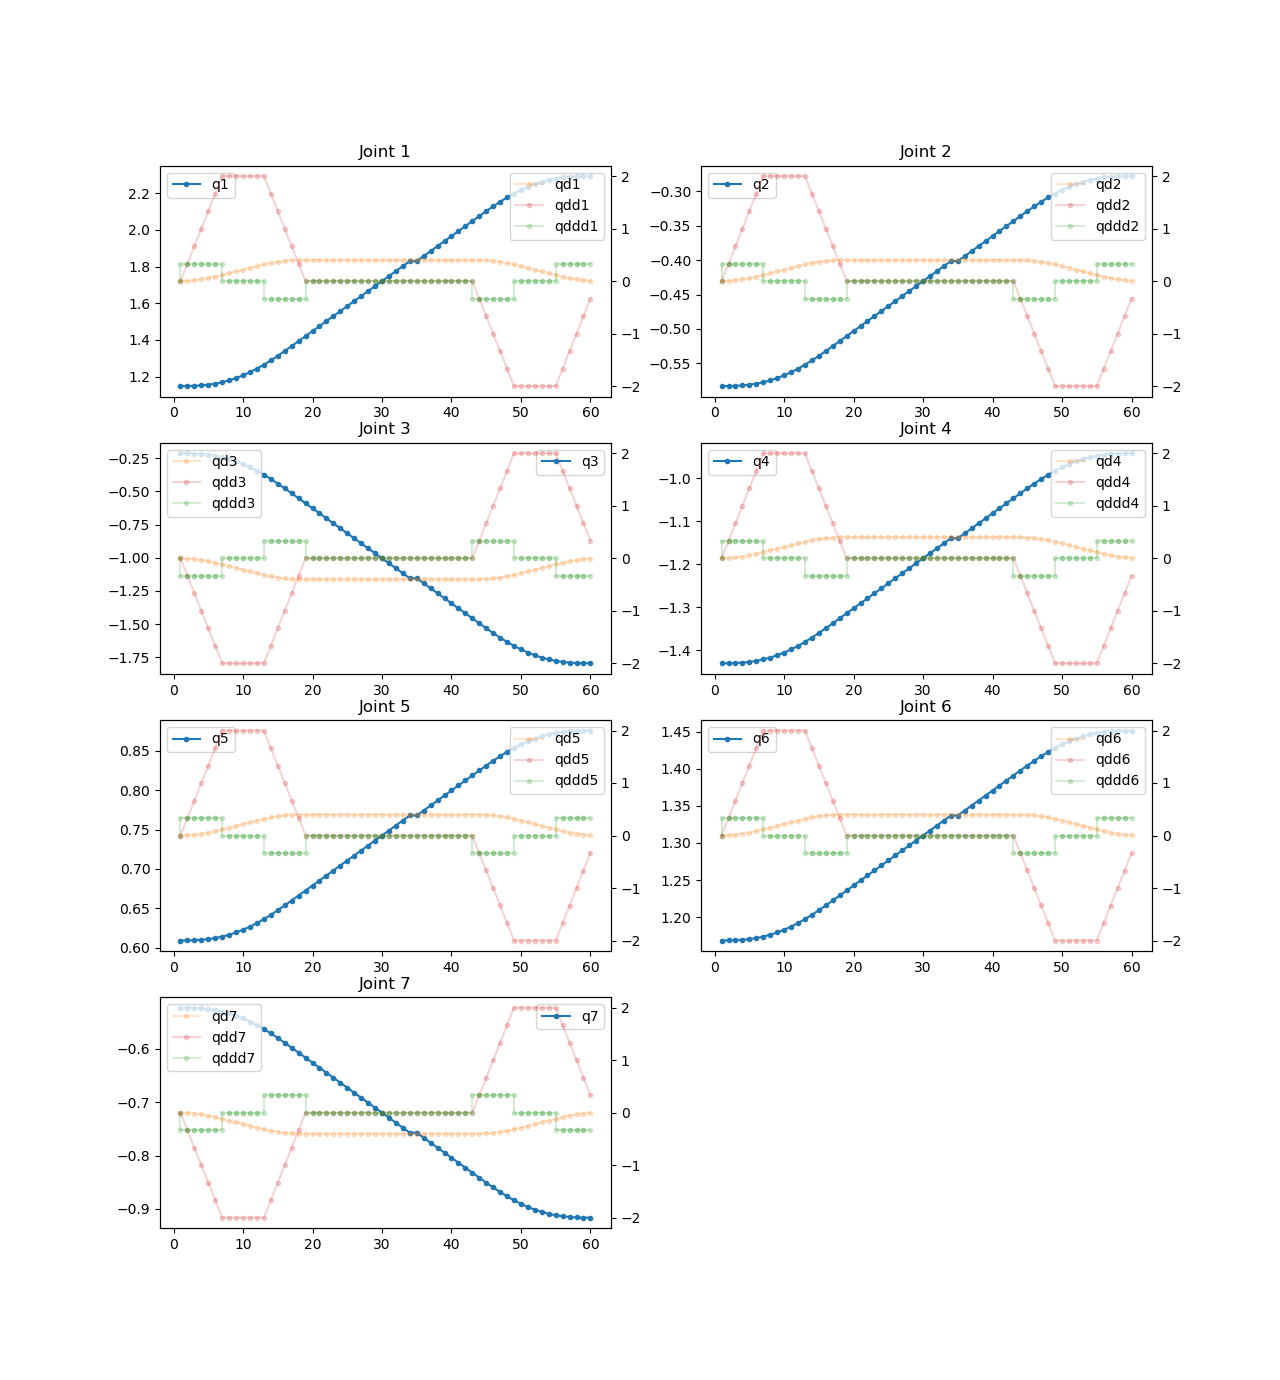
\includegraphics[width=\textwidth]{images/robot_planner3/3g_s_curve.png}
\caption{Experiment 3g: Trajectory using a s-curve velocity profile. The time constants are $τ_1 = τ_2 = 6$ seconds and the total trajectory duration is 60 seconds. The trajectory is computed at 60 sampling points.}
\label{robot-planner3g-joint-s-curve}
\end{figure}
\end{center}


\subsection{Helical trajectories in task space}

The goal of this experiment is to generate a helical trajectory inside the surgical taskspace which will then be transformed via the fulcrum transformation 
to a trajectory that the robotic arm can execute. To define a helical trajectory in the taskspace, two parameters are required: the $(x,y,z)$ coordinates of the 
helix center, it's radius $r$, as well as the number of cycles $τ$ of the helix and slope parameter $β$.\\ 

\begin{center}
\begin{figure}[!htb]
\centering
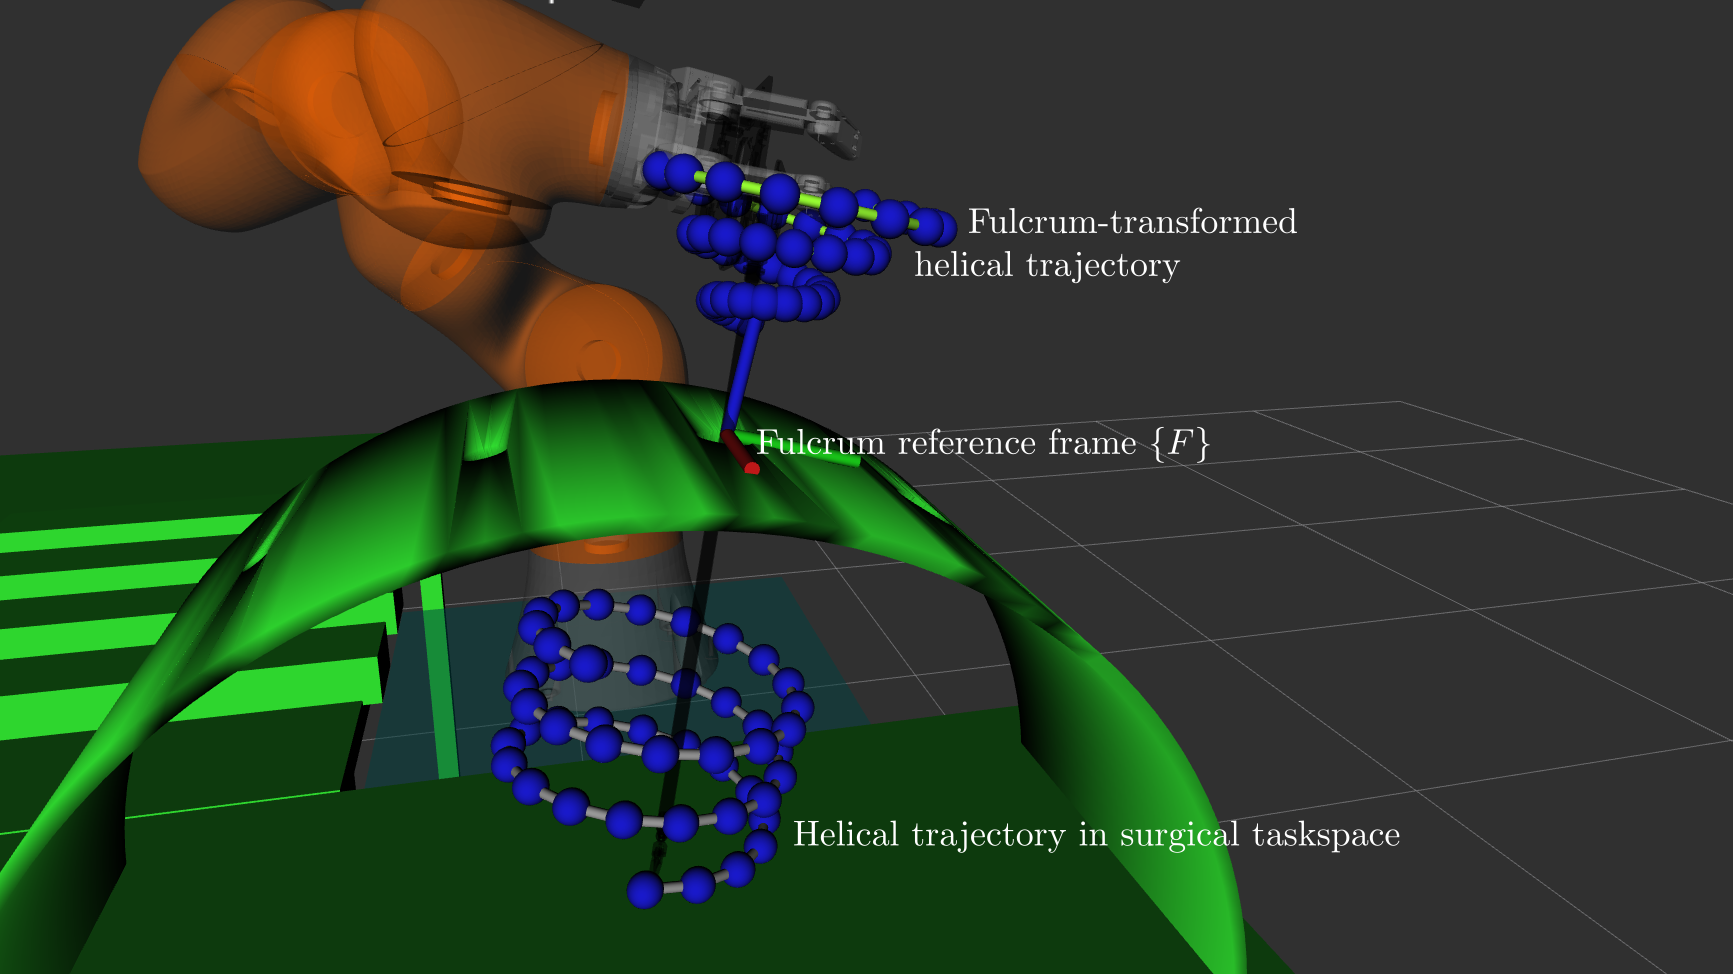
\includegraphics[width=\textwidth]{images/robot_planner3/3h_helix.png}
\caption{Experiment 3h: Create helical trajectory inside the surgical site (below the green mounting dock) and transform it via the fulcrum transformation to a trajectory for the robot's TCP.}
\label{robot-planner3h-helix}
\end{figure}
\end{center}


\section{Robot Planner 4: Simple cube pick-and-place experiment}

In this experiment we plan a simple pick-and-place path for a cube. The robotic arm first visits the left table and starts from the pre-grasp posture and then 
slowly approaches the cube until the grasp posture. When the gripper has reached the grasp posture, it closes the fingers to grasp the object and then retreats 
to the post-grasp posture. After that the robotic arm visits the right table to execute the place steps which are similar to the pick steps. The images below 
show some frames from the experiment with the first three to show the pick steps in the simulation environment and then other three images show the place steps 
in the visualization program.

\begin{center}
\begin{figure}[!htb]
\centering
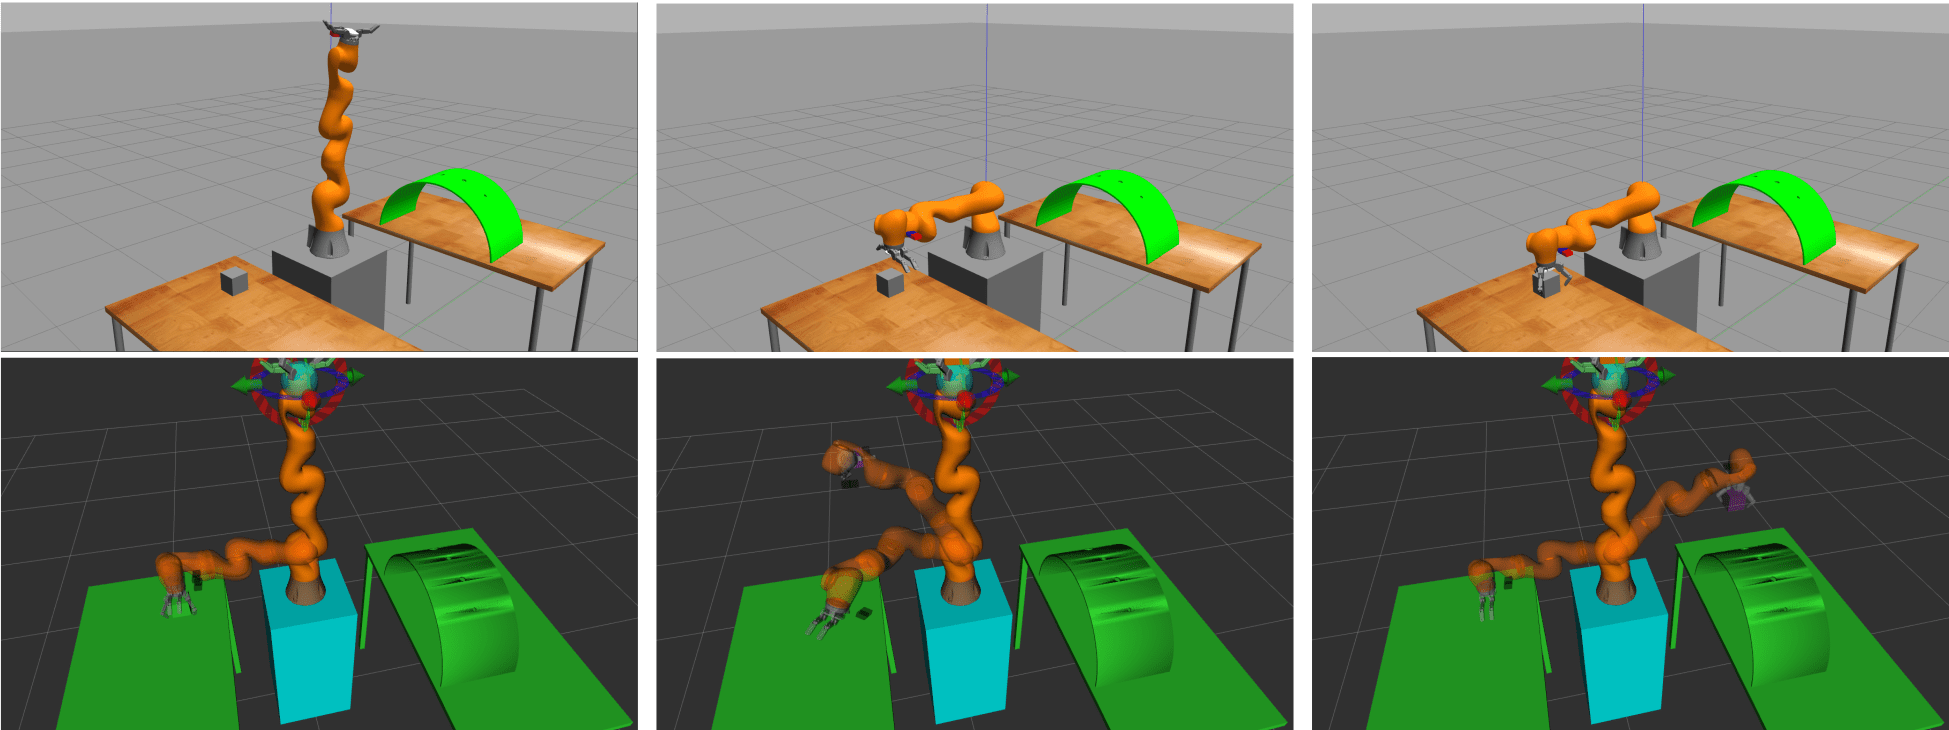
\includegraphics[width=\textwidth]{images/robot_planner4/robot_planner4}
\caption{Experiment 4: Simple pick-and-place experiment of a cube}
\end{figure}
\end{center}

Observing the results from table \ref{robot-planner4-rrtconnect-data}, the time duration for the pick pipeline of this experiment using the RRTConnect path planning algorithm, 
ranges from approximately 0.01 to 0.02 seconds, whereas in the Place pipeline we observe mainly 2 distinct groups of time ranges. One group has values around 0.02 seconds and the other 
has bigger values around 0.14 seconds. In the case with the bigger time durations, the solution made the robot go around the obstacle whereas in the other cases the path planning solution avoided the obstacle, 
which means that an easier path was found, it was solved quicker and the path solution was much simpler (in terms of kinematic constraints) which led to smaller path simplification time durations. 
It is also possible, that due to the obstacle and the initial conditions, the robot may not find a solution at the first attempt or none at all.

% Robot Planner 4 with RRTConnect
\begin{longtable}{|p{2cm}|c|p{3cm}|p{3cm}|p{3cm}|}
\hline
Robot Planner 4           & \multicolumn{4}{c}{\textbf{RRTConnect}}                                                                                                 \vline \\
\hline
                          & \multicolumn{4}{c}{\textbf{Pick Pipeline}}                     \vline \\
\hline
Experiment                & Status & Solution Time & Path Simplification Time & Planning Attempts  \\
\hline
1 & 1 & 0.026189 & 0.065173 & 1 \\
2 & 1 & 0.016835 & 0.043333 & 1 \\
3 & 1 & 0.025439 & 0.023178 & 1 \\
4 & 1 & 0.029292 & 0.066913 & 1 \\
5 & 1 & 0.024873 & 0.01747 & 1 \\
6 & 1 & 0.017615 & 0.024568 & 1 \\
7 & 1 & 0.014263 & 0.028095 & 1 \\
8 & 1 & 0.015479 & 0.027035 & 1 \\
9 & 1 & 0.027803 & 0.057064 & 1 \\
10 & 1 & 0.026057 & 0.033179 & 1 \\
\hline
\textbf{Average} & 1	& 0.02196178	& 0.0386008	& 1 \\
\hline
                          & \multicolumn{4}{c}{\textbf{Place Pipeline}}                     \vline \\
\hline
Experiment                & Status & Solution Time & Path Simplification Time & Planning Attempts  \\
\hline
1 & 1 & 0.014644 & 0.020947 & 1 \\
2 & 1 & 0.131334 & 0.938948 & 1 \\
3 & 1 & 0.021425 & 0.08429 & 1 \\
4 & 1 & 0.01675 & 0.01675 & 1 \\
5 & 1 & 0.165795 & 1.661019 & 1 \\
6 & 1 & 0.119819 & 0.394493 & 1 \\
7 & 1 & 0.140645 & 0.476835 & 1 \\
8 & 1 & 0.133917 & 0.673233 & 1 \\
9 & 1 & 0.017644 & 0.038319 & 1 \\
10 & 1 & 0.020025 & 0.074847 & 1 \\
\hline
\textbf{Average} & 1	& 0.0781998	& 0.4379681	& 1 \\
\hline
\caption{Time results for robot planner 4 using the RRTConnect path planner algorithm}
\label{robot-planner4-rrtconnect-data}
\end{longtable}

The main observation from the results of table \ref{robot-planner4-rrtstar-data} is that RRT* time durations are much bigger than those from RRTConnect, but the RRT* algorithm has the advantage of finding better, more accurate solutions (approximately the same solutions at most attempts) and with less collisions. Although these time durations are not optimal for real-time applications, they could be useful in pick-and-place pipelines 
if the solutions are pre-computed (memoized) and saved for later use.

% Robot Planner 4 with RRT*
\begin{longtable}{|p{2cm}|c|p{3cm}|p{3cm}|p{3cm}|}
\hline
Robot Planner 4           & \multicolumn{4}{c}{\textbf{RRT*}}                                                                                                 \vline \\
\hline
                          & \multicolumn{4}{c}{\textbf{Pick Pipeline}}                     \vline \\
\hline
Experiment                & Status & Solution Time & Path Simplification Time & Planning Attempts  \\
\hline
1	& 1 & 44.97476	& 0.030918	& 1	\\
2	& 1 & 45.006897	& 0.073009	& 1	\\
3	& 1	& 44.989085	& 0.053440	& 1	\\
4	& 1 & 44.998414	& 0.034571	& 1	\\
5	& 1 & 44.982524	& 0.041732	& 1	\\
6	& 1 & 44.997148	& 0.017660	& 1	\\
7	& 1 & 45.00115	& 0.022290	& 1	\\
8	& 1 & 44.991409	& 0.046728	& 1	\\
\hline
\textbf{Average} & 1 & 44.99267	& 0.0400435	& 1	\\
\hline
                          & \multicolumn{4}{c}{\textbf{Place Pipeline}}                     \vline \\
\hline
Experiment                & Status & Solution Time & Path Simplification Time & Planning Attempts  \\
\hline
1	& 1	& 45.064568	& 0.884821	& 1 \\
2	& 1	& 44.965931	& 0.054692	& 1 \\
3	& 1	& 44.976697	& 0.012784	& 1 \\
4	& 1	& 44.968431	& 0.020354	& 1 \\
5	& 1	& 45.068239	& 0.551800	& 1 \\
6	& 1	& 45.016043	& 1.089529	& 1 \\
7	& 1	& 45.048851	& 0.680121	& 1 \\
8	& 1	& 45.023364	& 0.000004	& 1 \\
\hline
\textbf{Average} & 1	& 45.0165155	& 0.411763	& 1 \\
\hline
\caption{Time results for robot planner 4 using the RRT* path planner algorithm}
\label{robot-planner4-rrtstar-data}
\end{longtable}

% Robot Planner 4 with PRM*
\begin{longtable}{|p{2cm}|c|p{3cm}|p{3cm}|p{3cm}|}
\hline
Robot Planner 4           & \multicolumn{4}{c}{\textbf{PRM*}}                                                                                                 \vline \\
\hline
                          & \multicolumn{4}{c}{\textbf{Pick Pipeline}}                     \vline \\
\hline
Experiment                & Status & Solution Time & Path Simplification Time & Planning Attempts  \\
\hline
1	& 1	& 44.987182	& 0.000028	& 1 \\
2	& 1	& 44.992757	& 0.000005	& 1 \\
3	& 1	& 45.00983	& 0.000004	& 1 \\
4	& 1	& 45.004154	& 0.105568	& 1 \\
5	& 1	& 44.99367	& 0.000002	& 1 \\
6	& 1	& 45.015169	& 0.000002	& 1 \\
7	& 1	& 45.02914	& 0.000002	& 1 \\
\hline
\textbf{Average} & 1	& 45.00456	& 0.015088	& 1 \\
\hline
                          & \multicolumn{4}{c}{\textbf{Place Pipeline}}                     \vline \\
\hline
Experiment                & Status & Solution Time & Path Simplification Time & Planning Attempts  \\
\hline
1	& 1	& 44.992207	& 0.000004	& 1 \\
2	& 1	& 45.512132	& 0.000001	& 1 \\
3	& 1	& 45.950533	& 0.000002	& 1 \\
4	& 1	& 44.99777	& 0.000003	& 1 \\
5	& 1	& 45.691226	& 0.000002	& 1 \\
6	& 1	& 45.023251	& 0.013478	& 1 \\
7	& 1	& 45.782305	& 0.000003	& 1 \\
\hline
\textbf{Average}	& 1	& 45.421346	& 0.0019276	& 1 \\
\hline
\caption{Time results for robot planner 4 using the PRM* path planner algorithm}
\label{robot-planner4-prmstar-data}
\end{longtable}


\section{Robot Planner 5: Visual servoing}

The goal of this fifth experiment is to control the KUKA robot using the camera via the visual servoing technique. In the first part of the experiment the 
robotic arm goes to an initial known position (e.g. the corner of the table) and then moves around until it detects a surgical tool. When that happens, the 
image-based visual servoing will send commands to the robot so that the detected tool is at the center of the video frame and with the same orientation 
as the video frame. At the second part of the experiment, the robot follows a similar algorithm. It starts with a known position, like the corner of the second 
table, then moves around until the mounting dock starts to appear inside the frame. When that happens, the image-based visual servoing will send commands to the 
robot so that the center of the trocar or the fulcrum reference frame is at the center and with the same orientation as the video frame. Similar results can be 
achieved by using position-based visual servoing, but that was not chosen at this implementation for simplicity and less operations. Position-based servoing 
requires more calculations because it is required to get the camera's transformation, express it with respect to the end-effector and then calculate the 
end-effector pose which is then used as an input to a Cartesian Controller.

\begin{center}
\begin{figure}[H]
\centering
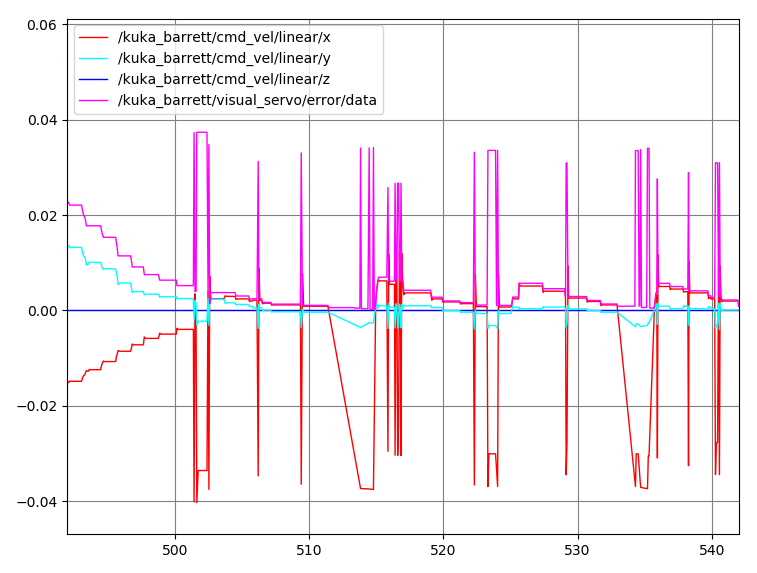
\includegraphics[width=0.45\textwidth]{images/robot_planner5/visual_servo_controller3.png}
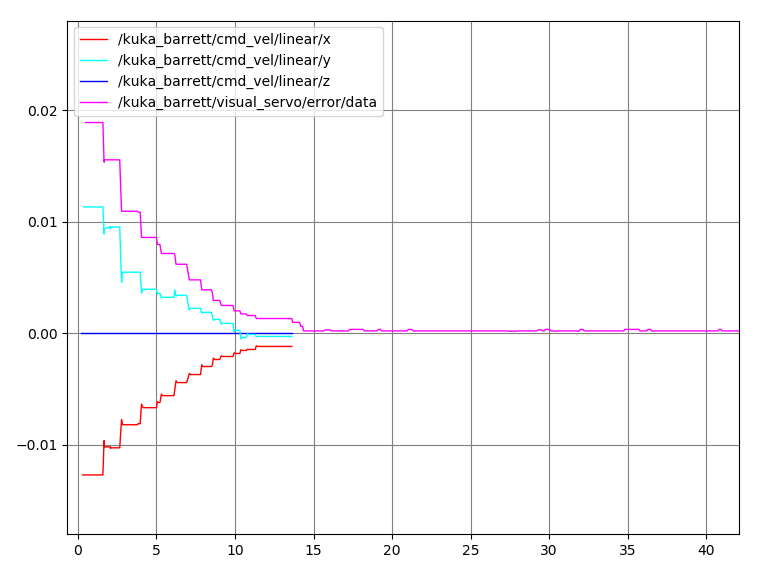
\includegraphics[width=0.45\textwidth]{images/robot_planner5/visual_servo_controller4.png}\\
\caption{Visual servo controller error diagrams. On the left image in the error graphs appear some spikes. These spikes occur from the sudden temporary detection 
of a nearby surgical tool. On the right image, these spikes are filtered out, and only the error graphs of the visual servoing of one tool are shown. The  
controller parameters are $K_p = 0.9, K_d = 0.2$}
\end{figure}
\end{center}

\begin{center}
\begin{figure}[!htb]
\centering
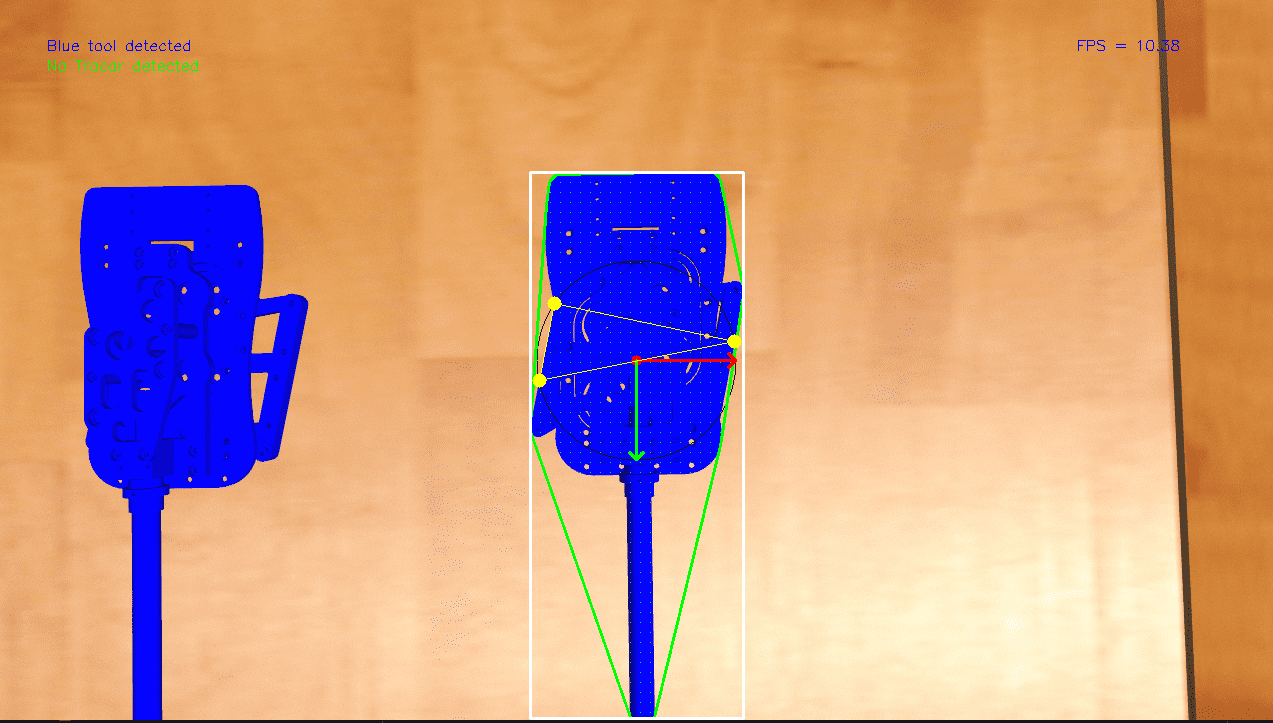
\includegraphics[width=0.6\textwidth]{images/grasp-points-triangle.png}\\
\caption{Image based visual servoing and calculation of grasp points. The yellow points are the grasp points and the thin black circumscribed circle is the growing circle that was used to calculate them.}
\end{figure}
\end{center}



\section{Robot Planner 6: RCM alignment error in insertion and retraction}

The goal of this experiment is to measure the alignment error of the long axis of the surgical tool with the fulcrum point. This error tracks whether the robot pose satisfies the RCM constraint, 
in which the axis of the tool must always pass through the fulcrum point and is explained in more detail in \ref{section:rcm-tracking}. To simplify the experiment, 
constant values are assumed for both position coordinates and orientation angles and a constant arbitrary diagonal covariance matrix.
\begin{equation}
\begin{bmatrix}
x \\ y \\ z \\ ψ \\ θ \\ φ \\
\end{bmatrix} = 
\begin{bmatrix}
0.529996 \\ 0.059271 \\ 1.398114 \\ -0.271542 \\ 0 \\ 0 \\
\end{bmatrix}, \quad \mathbf{C} = diag(0.001, \cdots, 0.001)
\end{equation}
where $\mathbf{p} = [x,y,z]$ and the Euler angles $ψ, θ, φ$ are later used to calculate the quaternion $\mathbf{q}$. \\

\begin{center}
\begin{figure}[!htb]
\centering
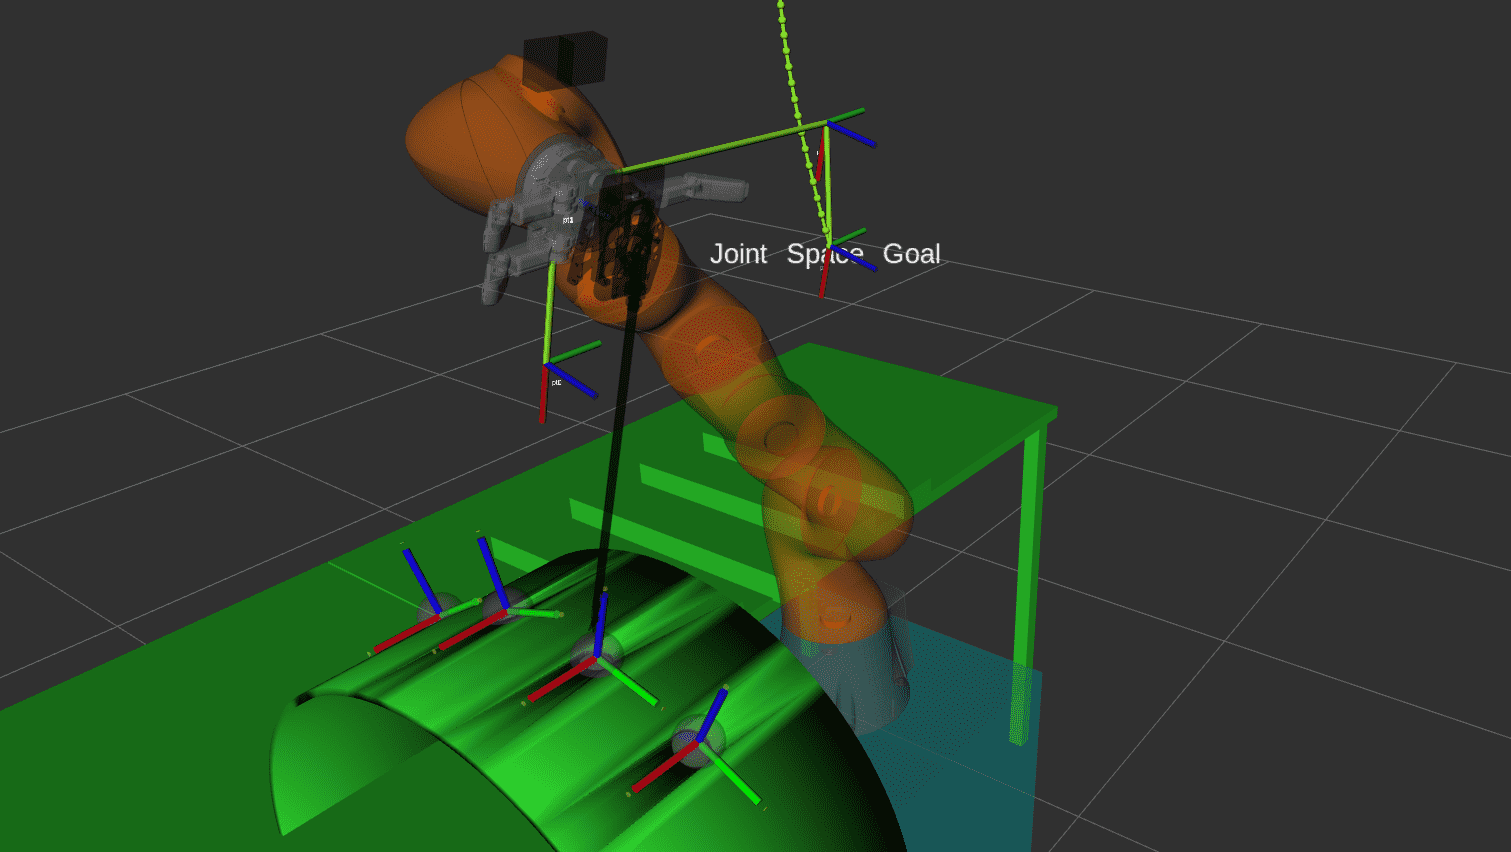
\includegraphics[width=\textwidth]{images/robot_planner6/robot_planner6.png}
\caption{Robot planner6: Path from home, to point above Fulcrum point and path of insertion/retraction}
\end{figure}
\end{center}

\begin{center}
\begin{figure}[!htb]
\centering
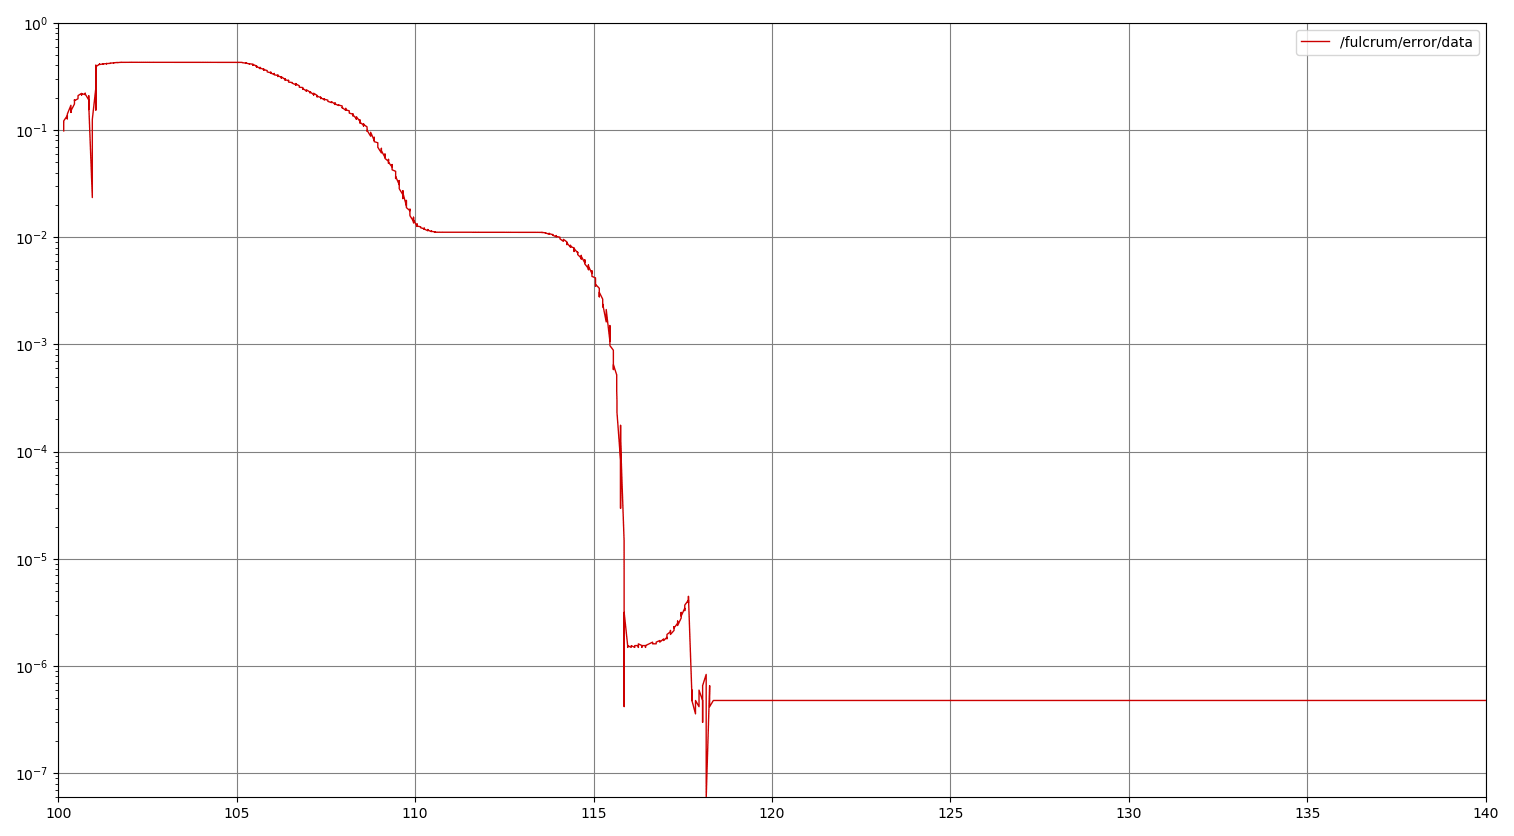
\includegraphics[width=\textwidth]{images/robot_planner6/rcm_fulcrum_alignment_error.png}
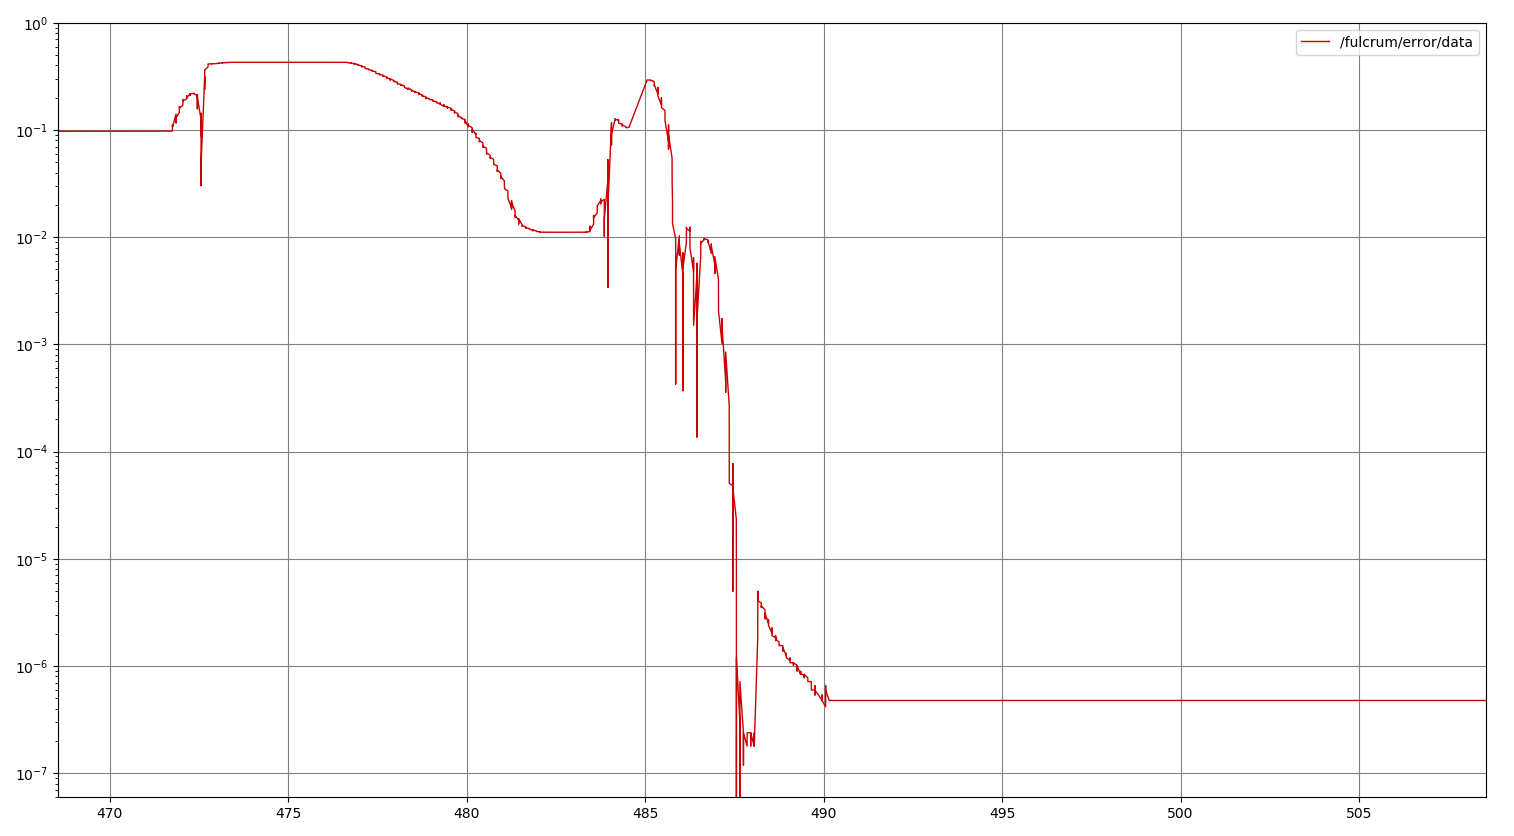
\includegraphics[width=\textwidth]{images/robot_planner6/rcm_fulcrum_alignment_error2.png}\\
\caption{RCM alignment error, diagrams from 2 executions of the same experiment. The x-axis is measured in seconds (ROS time) and the y-axis is the distance error measured in meters in logarithmic scale.}
\end{figure}
\end{center}

\begin{center}
\begin{figure}[!htb]
\centering
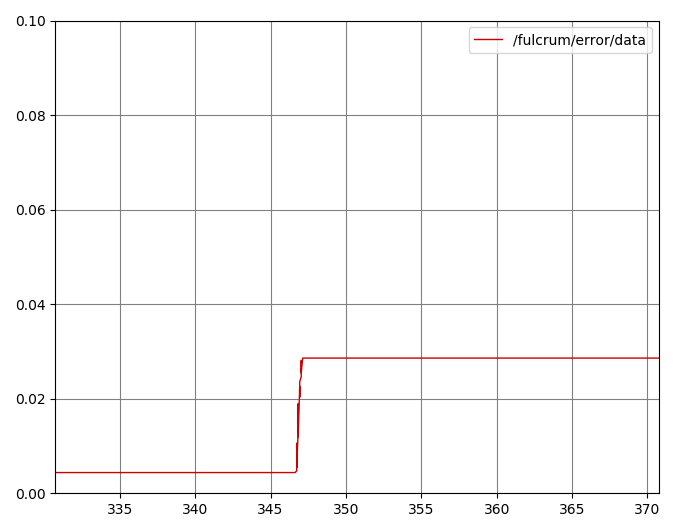
\includegraphics[width=0.49\textwidth]{images/robot_planner6/rcm-error-collision.png}
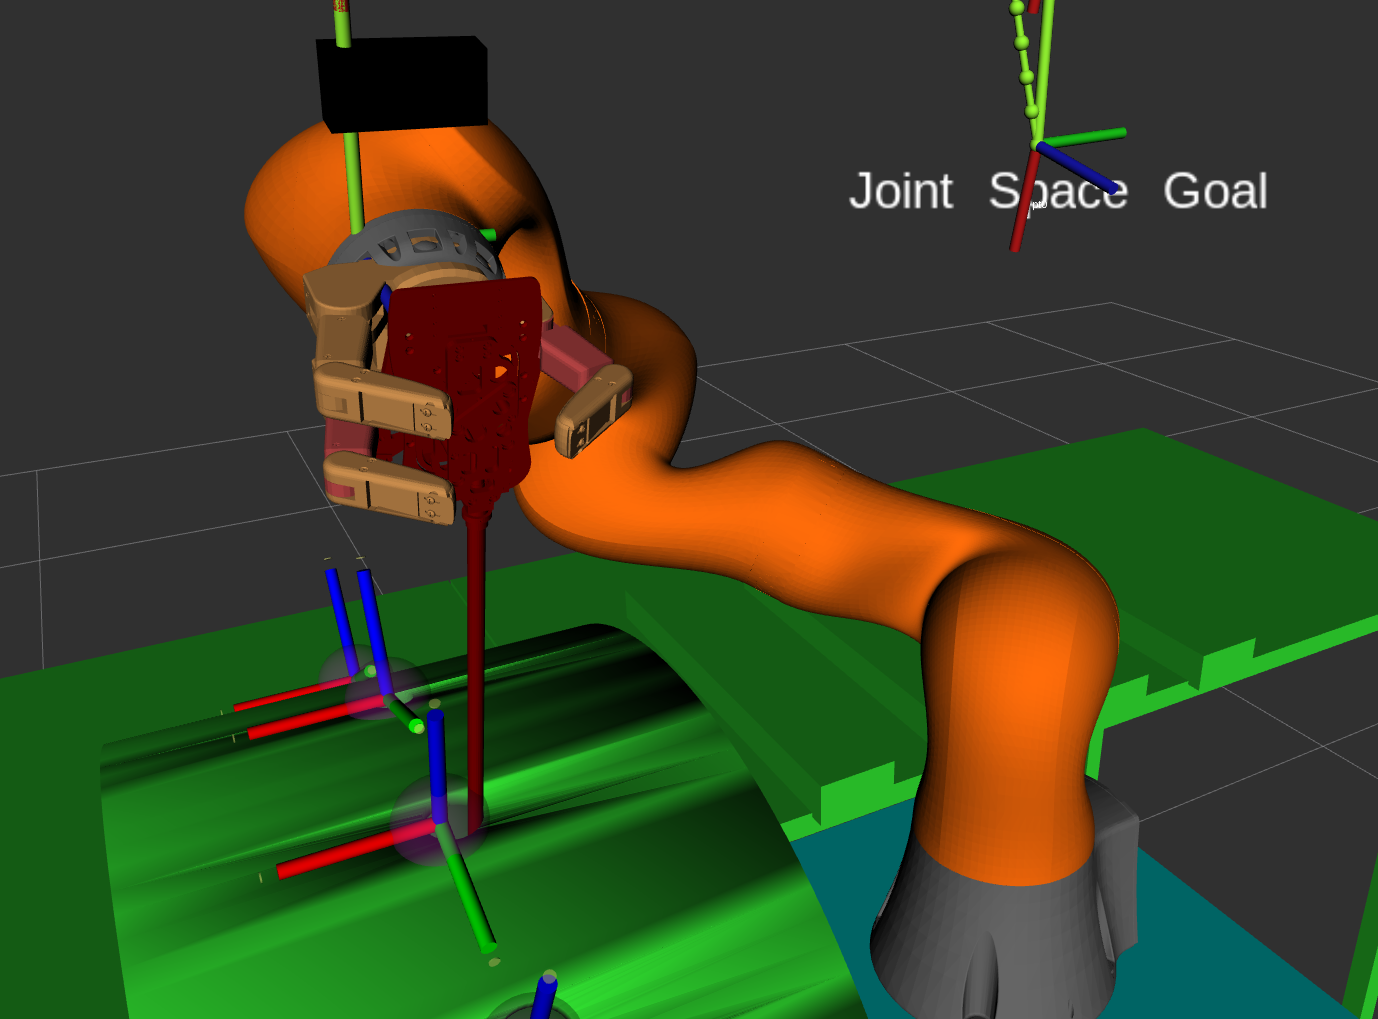
\includegraphics[width=0.49\textwidth]{images/robot_planner6/rcm-collision.png}\\
\caption{Surgical tool slides from an aligned, RCM pose to a pose misaligned from the fulcrum point, no RCM motion and surgical tool is is collision, exerting pressure to the abdominal wall. The diagram on the 
left shows the error starting from a correct position to a problematic position. The right image shows the tool in collision with the mounting dock (abdominal wall) and there is an obvious distance from the 
fulcrum reference frame.}
\end{figure}
\end{center}

\begin{center}
\begin{figure}[!htb]
\centering
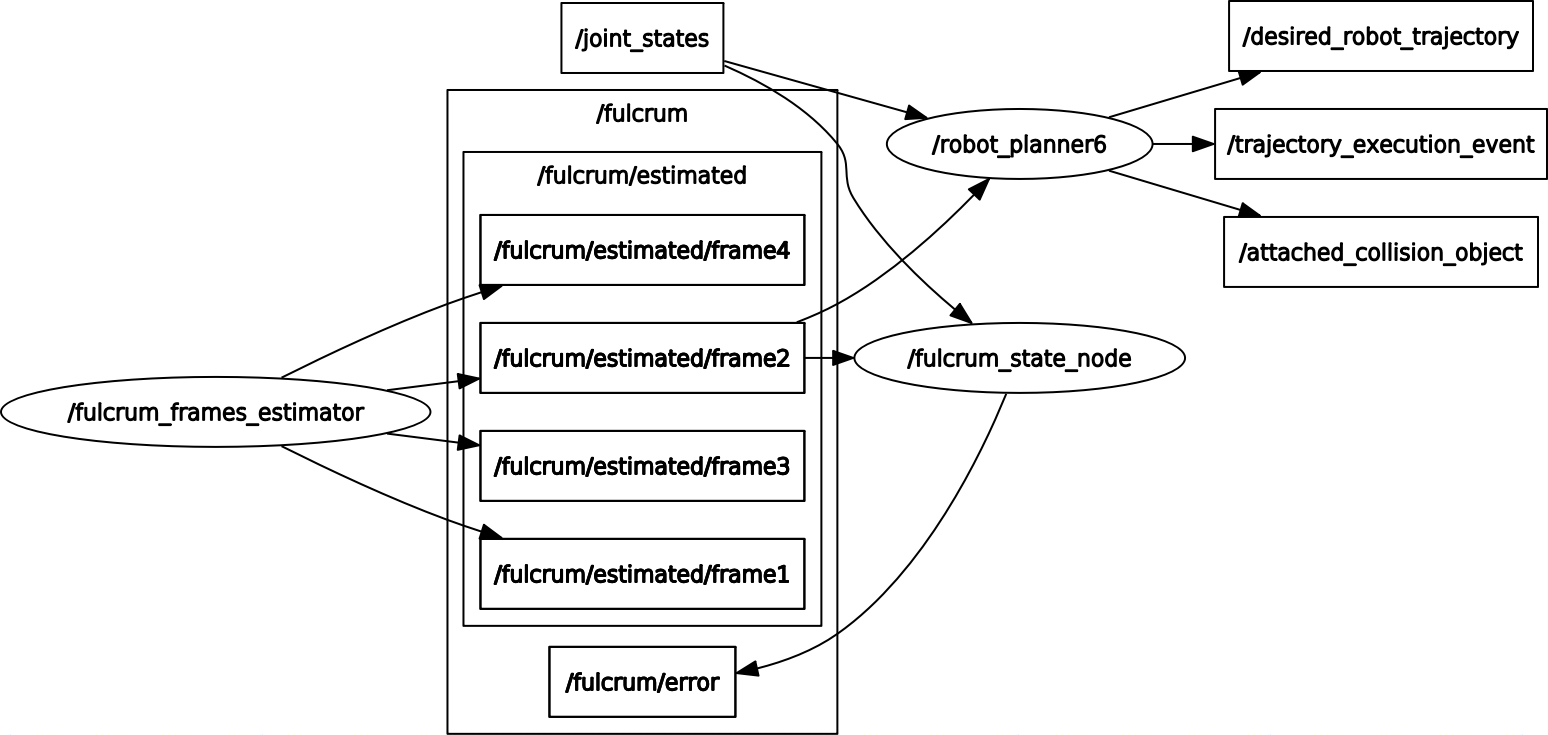
\includegraphics[width=\textwidth]{images/robot_planner6/topics-and-nodes.png}
\caption{ROS nodes and topics used for the robot-planner6 experiment. In this experiment the trajectories and RCM fulcrum errors are with respect to the 2nd fulcrum reference frame only.}
\end{figure}
\end{center}


\newpage
\section{Robot Planner 7: State machine - End-to-end running}
\label{section:robot-planner7}

The goal of this experiment is to run all stages of this thesis together to study the end-to-end result. Each stage is run by a different node and the sequence in which every task is executed is dictated by the status 
of the state machine as shown in figure \ref{smack-state-machine}.

\begin{center}
\begin{figure}[!htb]
\centering
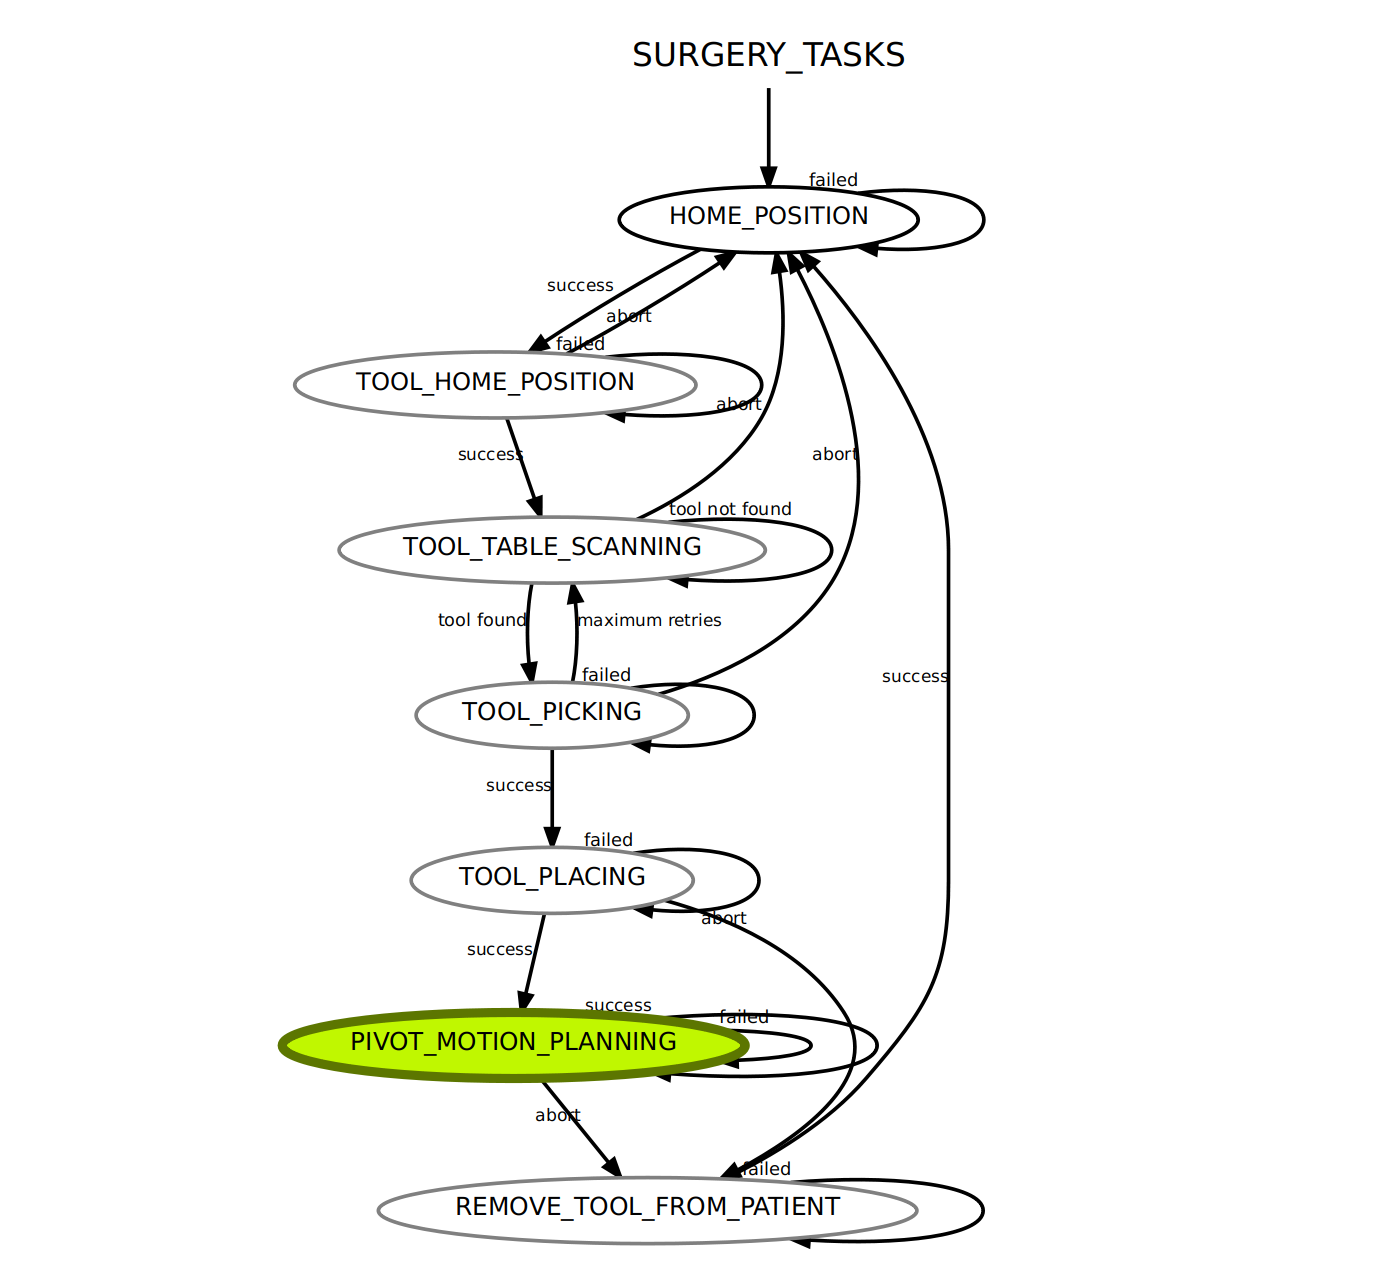
\includegraphics[width=\textwidth]{images/state-machine-all-tasks.png}
\caption{State machine status, shown in smach viewer}
\label{smack-state-machine}
\end{figure}
\end{center}